%%%%%%%%%%%%%%%%%%%%%%%%%%%%%%%%%%%%%%%%%
% Masters/Doctoral Thesis 
% LaTeX Template
% Version 1.42 (19/1/14)
%
% This template has been downloaded from:
% http://www.latextemplates.com
%
% Original authors:
% Steven Gunn 
% http://users.ecs.soton.ac.uk/srg/softwaretools/document/templates/
% and
% Sunil Patel
% http://www.sunilpatel.co.uk/thesis-template/
%
% License:
% CC BY-NC-SA 3.0 (http://creativecommons.org/licenses/by-nc-sa/3.0/)
%
% Note:
% Make sure to edit document variables in the Thesis.cls file
%
%%%%%%%%%%%%%%%%%%%%%%%%%%%%%%%%%%%%%%%%%

%----------------------------------------------------------------------------------------
%	PACKAGES AND OTHER DOCUMENT CONFIGURATIONS
%----------------------------------------------------------------------------------------

\documentclass[11pt, a4paper, oneside]{Thesis} % Paper size, default font size and one-sided paper

\graphicspath{{images/}} % Specifies the directory where pictures are stored

\hypersetup{urlcolor=black, colorlinks=true} % Colors hyperlinks in blue - change to black if annoying
\title{\ttitle} % Defines the thesis title - don't touch this

\begin{document}

\frontmatter % Use roman page numbering style (i, ii, iii, iv...) for the pre-content pages

\setstretch{1.3} % Line spacing of 1.3

\pagestyle{plain}

\newcommand{\HRule}{\rule{\linewidth}{0.5mm}} % New command to make the lines in the title page

% Subreferences Setup
\captionsetup{subrefformat=parens}

% PDF meta-data
\hypersetup{pdftitle={\ttitle}}
\hypersetup{pdfsubject=\subjectname}
\hypersetup{pdfauthor=\authornames}
\hypersetup{pdfkeywords=\keywordnames}

%----------------------------------------------------------------------------------------
%	DEFINITIONS OF NEW COMMANDS
%----------------------------------------------------------------------------------------

% vector variable command
\newcommand*\vecvar[1]{\mathbfit#1}

% matrix variable command
\newcommand*\matvar[1]{\mathbf#1}

% transpose command
\newcommand*\transpose[1]{#1^{T}}

% trace command
\newcommand*\trace[1]{Tr(#1)}

% Bernoulli distribution command
\newcommand*\bernoulli[1]{Be(#1)}

% i.i.d. command
\newcommand*\iid{i.i.d.\xspace}

% probability event command
\newcommand*\probability[1]{\Pr(#1)}

% expectation command
\newcommand*\expectation[1]{\mathbb{E}(#1)}

% variance command
\newcommand*\variance[1]{Var(#1)}

% covariance command
\newcommand*\covariance[2]{Cov(#1#2)}

% graph variable command
\newcommand*\graphvar[1]{\mathcal#1}

% set variable command
\newcommand*\setvar[1]{\mathcal#1}

% cardinality set command
\newcommand*\cardinality[1]{\left\vert#1\right\vert}

% mean command
\newcommand*\mean[1]{\langle#1\rangle}

% absolute value command
\newcommand*\abs[1]{\left\vert#1\right\vert}

% emphasise in text command
\newcommand*\emphT[1]{\textit{#1}}

% natural logarithm command
\newcommand*\natlog[1]{\log#1}

% euler constant (e) command
\newcommand{\euler}{e\xspace}

% set of real numbers 'R' command
\newcommand*\realsR{\mathbb{R}\xspace}

% special number one (1) command
\newcommand*\one{\mathds{1}\xspace}

%optimizaiton 
\newcommand*{\argmax}{\operatornamewithlimits{argmax}\limits}

%----------------------------------------------------------------------------------------
%	TITLE PAGE
%----------------------------------------------------------------------------------------

\begin{titlepage}
\begin{center}


\includegraphics[scale=0.1]{imperialCrest} % University/department logo - uncomment to place it 

\textsc{\LARGE \univname}\\[1cm] % University name
\textsc{\Large Final Year Project Report}\\[0.5cm] % Thesis type

\HRule \\[0.4cm] % Horizontal line
{\huge \bfseries \ttitle}\\[0.1cm] % Thesis title
\HRule \\[1.5cm] % Horizontal line
 
\begin{minipage}{0.4\textwidth}
\begin{flushleft} \large
\emph{Author:}\\
{\authornames} % Author name - remove the \href bracket to remove the link
\end{flushleft}
\end{minipage}
\begin{minipage}{0.4\textwidth}
\begin{flushright} \large
\emph{Supervisor:} \\
{\supname} \\% Supervisor name - remove the \href bracket to remove the link
\emph{Second marker:} \\
{\secmark}
\end{flushright}
\end{minipage}\\[2cm]
 
\large This report is submitted in fulfilment of the requirements\\ for the degree of \textit{\degreename}\\ % University requirement text
in the\\
\deptname\\\univname\\[1.5cm] % Research group name and department name

{\large \today}\\[0.1cm] % Date

\vfill
\end{center}

\end{titlepage}

% blank page
\thispagestyle{empty}
\mbox{}
\newpage

%----------------------------------------------------------------------------------------
%	ABSTRACT PAGE
%----------------------------------------------------------------------------------------

\addtotoc{Abstract} % Add the "Abstract" page entry to the Contents

\abstract{Write Abstract here...}

\clearpage % Start a new page

%----------------------------------------------------------------------------------------
%	ACKNOWLEDGEMENTS
%----------------------------------------------------------------------------------------

\setstretch{1.3} % Reset the line-spacing to 1.3 for body text (if it has changed)

\acknowledgements{Write Acknowledgements here...}

\clearpage % Start a new page

%----------------------------------------------------------------------------------------
%	LIST OF CONTENTS/FIGURES/TABLES PAGES
%----------------------------------------------------------------------------------------

\tableofcontents

\listoffigures

\listoftables


%----------------------------------------------------------------------------------------
%	NOTATIONS
%----------------------------------------------------------------------------------------

\clearpage % Start a new page

\setstretch{1.3} % Reset the line-spacing to 1.3 for body text (if it has changed)

\listofnomenclature{ll}
{
$\cardinality{\setvar{S}}$ & Cardinality of the set $\setvar{S}$ \\
$\one_{\setvar{S}}$ & Indicator variable over the set $\setvar{S}$ \\
$y$ & Scalar $y$ \\
$\abs{y}$ & Absolute value of $y$ \\
$\vecvar{v}$ & Vector $\vecvar{v}$ \\
$\matvar{M}$ & Matrix $\matvar{M}$ \\
$M_{ij}$ & The element of the matrix $\matvar{M}$ at row $i$ and column $j$\\
$\transpose{\matvar{M}}$ & Transpose of the matrix $\matvar{M}$ \\
$\abs{\matvar{M}}$ & Determinant of the matrix $\matvar{M}$ \\
$\trace{\matvar{M}}$ & Trace of the matrix $\matvar{M}$ \\
$\expectation{X}$ & Expected value of $X$ \\
$\variance{X}$ & Variance of $X$ \\
$\natlog(x)$ & \emphT{natural logarithm} of $x$ (logarithm to the base $\euler$)
}

%----------------------------------------------------------------------------------------
%	THESIS CONTENT - CHAPTERS
%----------------------------------------------------------------------------------------



\mainmatter % Begin numeric (1,2,3...) page numbering

\nocite{*}

% Introduction
%\tableofcontents{}
\chapter{Introduction}
\label {sec:introduction}
Computer vision, a relative new area of research has risen with the growth of technology for the past decade. It is an emerging science which involves teaching machines or computers to see and make decisions and judgements. As discussed in \cite{EGL}, goals of computer vision can be divided into different categories as engineering and way to understand intelligence. Real world applications like surveillance, photography and navigation have been developed and put into use gradually. By applying machine learning techniques, applications can be designed and built to meet varies needs. Although computer vision has a lot of potential applications and is much more efficient than human as the digital data size grows tremendously every year, it has been considered difficult because it frequently fails in accuracy to human visual system by comparison. 

For instance, a human can distinguish between body parts of different people under almost any circumstances which are not too extreme. However, a computer may not be able to easily achieve this kind of task due various conditions such as light illumination, viewpoints and different gestures. Therefore, how to represent human knowledge in computers and carry out real time computation efficiently and accurately have become the biggest challenges in the area of computer vision. Moreover, vision techniques are very domain dependent. Some approaches may fail in one specialized application but work well in other specified areas. \cite{EGL}. 

Face is a key subject in the area of object detection. Especially face recognition, which is an technology used to verify people's identity is very widely used in various fields such as security authentication systems, search potential criminals in urban area and unlocking smart phones. And research conducted on this subject is getting more and more important. In this project, we will try to address some sub-problems in facial recognition.

This report will emphasis on the state of the art machine learning algorithm known as random forest, which will be mentioned in detail in section \ref{sec:RF} and will be used to tackle problems such as head pose estimation in section \ref{sec:HPestimation} and face feature points detection in section \ref{sec:FLL} respectively.

% Background
\chapter{Background}
\label{sec:background}
In this section, the main algorithm used for this project will be mentioned as well as preliminaries regarding to computer vision.
\section{Computer Vision Preliminaries}
\label{sec:cvpre}
Before I go in to the details, let me introduce some necessary fundamentals.
\subsection{Image Format}
\label{sec:imageformat}
As far as this report is concerned, both RGB and depth images are used. RGB images have three channels, namely red, green and blue. Each of which has a value ranges from 0 to 255 which represents the respective intensity. The combination of the three channels will represent a pixel in a digital image. Unlike RGB, Grayscale (also know as black and white) images have only one channel and only possess the intensity information of a pixel. \cite{gray} 

The conversion from RGB to grayscale by the Luminosity method is :
\begin{equation}
 Grayscale = 0.21\times Red + 0.72\times Green + 0.07\times Blue
\end{equation}

Examples of a RGB image and it's corresponding Grayscale are shown in Figures \ref{fig:rgb} and \ref{fig:gray}

\begin{figure}
	\centering
	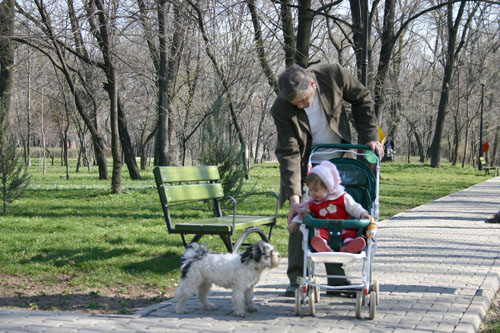
\includegraphics[width=0.8\linewidth]{Channel_digital_image_RGB_color.jpg}
	\caption[rgb image]{\label{fig:rgb}}  \textbf{RGB} 
\end{figure}

\begin{figure}
	\centering
	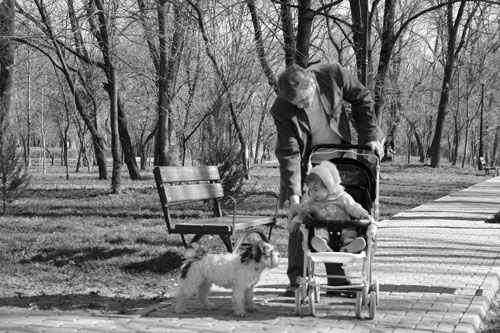
\includegraphics[width=0.8\linewidth]{Channel_digital_image_red.jpg}
	\caption[gray image]{\label{fig:gray}}  \textbf{Gray} 
\end{figure}

In addition to 2D images, due to the rise of depth sensor such as Microsoft Kinect. Depth images become available. Each pixel of a depth image contains the information of the distance from an object in a 3D scene to the viewpoint. An example of a depth image with its colour version is shown in Figure \ref{fig:depth}.

\begin{figure}
	\centering
	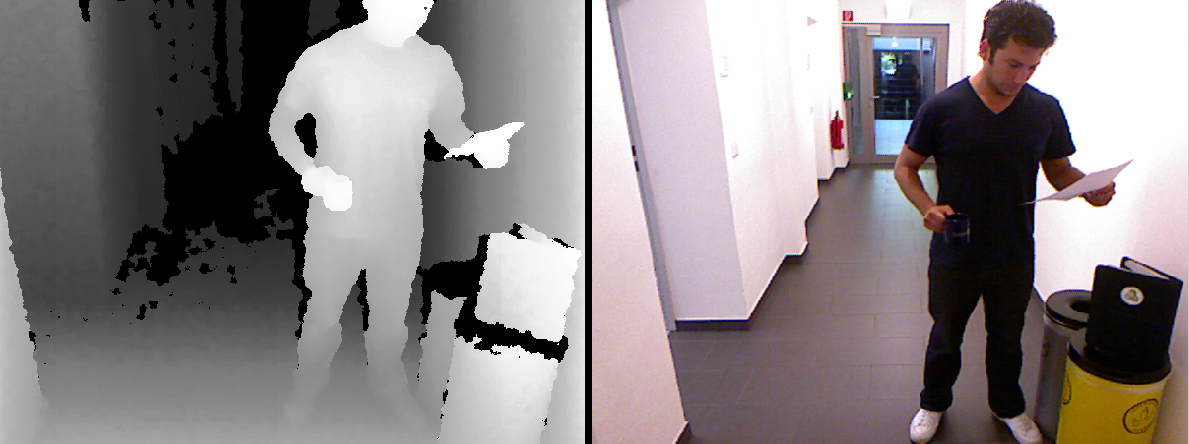
\includegraphics[width=0.8\linewidth]{depthandcolor.png}
	\caption[depth and colour images]{\label{fig:depth}}  \textbf{Depth and Colour} 
\end{figure}

\subsection{Euler Angles}
\label{sec:eulerangles}
Euler Angles are the most commonly used rotational coordinates. As far as this project is concerned, Euler angles are used to classify the head rotations. As shown in Fig \ref{fig:eulerangles}

\begin{figure}
	\centering
	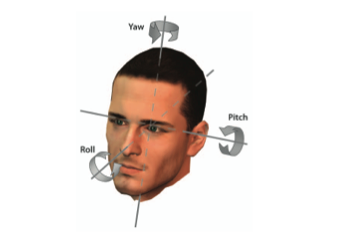
\includegraphics[width=0.8\linewidth]{headpose1.png}
	\caption[Euler Angles]{\label{fig:eulerangles}}  \textbf{"The three degrees of freedom of a human head can be described by the egocentric rotation angles pitch, roll, and yaw "\cite{HPS}} 
\end{figure}


%\section{Face Image analysis applications}
%\label{sec:faceapp}


%\section{General Object Detection Methods}
%\label{sec:objectD}
\newpage
\thispagestyle{plain}
\mbox{}

\section{Haar-Like Features}
\label{sec:HLfeatures}
The use of Haar-Like feature (as shown in Fig \ref{fig:hlfeature}) plays a big role in the scene of object detection. As mentioned in \cite{facedetect}, feature based systems perform better than pixel base systems. It is also known as rectangular features. In this project, only two rectangle feature is used which computes the difference between the sum of the pixels of two rectangular regions. One may notice, as the size of the rectangular region grows, the computation time will increase dramatically. Integral image is introduced to overcome this problem. \cite{facedetect}

\begin{figure}
	\centering
	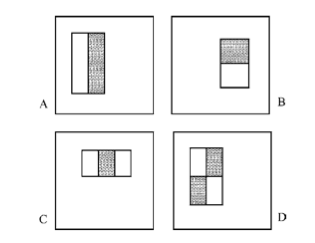
\includegraphics[width=0.6\linewidth]{hlfeature.png}
	\caption[Haar like Feature]{\label{fig:hlfeature}}  \textbf{A, B show the two rectangular feature whereas C and D show three rectangular feature and four rectangular feature respectively. The sum of the pixel values in the white rectangle is subtracted from the sum of the pixel values in the grey one. } \cite{facedetect}
\end{figure}

\subsection{Integral Image}
\label{sec:integralimage}
Feature computation is an important and necessary step in face image analysis but it could also be very time consuming as the size of the rectangular regions increase. As a result, integral image is used which enables fast computation. An integral image at location x, y contains the sum of the pixels above and to the left of x and y.(See Fig \ref{fig:integral1} \cite{integralimage} Analytically : 
\begin{equation}
sum(x,y)= \sum\limits_{a\leq x,b\leq y}i(a,b)
\end{equation}
Where $sum(x,y)$ is the pixel value at position (x,y) of the integral image and $i(a,b)$ is the pixel value at position (a,b) of the original image. Once integral images are created, sum within any rectangle can be computed by only referencing four points in the integral image. As shown in Fig \ref{fig:integral2}.

\begin{figure}
	\centering
	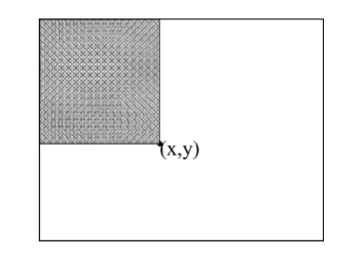
\includegraphics[width=0.6\linewidth]{integral1.png}
	\caption[Integral image]{\label{fig:integral1}}  \textbf{The value of the integral image at point(x,y) is the sum of all the pixels above and to the left  } \cite{integralimage}
\end{figure}

\begin{figure}
	\centering
	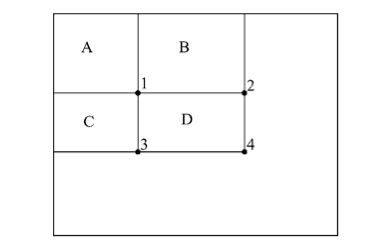
\includegraphics[width=0.6\linewidth]{integral2.png}
	\caption[Integral image referencing]{\label{fig:integral2}}  \textbf{If we are required to computer the sum of all the pixel values in D, the only 4 points we need to know is 1,2,3,4 since the value at 1 is A, the value at 2 is A + B, the value at 3 is A + C and the value at 4 is A + B + C + D, with a bit of algebra, it is not difficult to see that D = 4 + 1 - 2 - 3. }\cite{integralimage} 
\end{figure}

\newpage
\thispagestyle{plain}
\mbox{}

\section{AdaBoost}
\label{sec:adaboost}
In general, AdaBoost is an algorithm used to construct a strong classifier by combining number of weak classifiers as a weighted sum:
\begin{equation}
F(x) = \sum\limits_{t=1}^{T}\alpha_{t}h_{t}(x)
\end{equation}
Where $F(x)$ is the final strong classifier and $h_{t}(x), alpha_{t}$ are weak classifiers and their respective weights. The general Adaboost algorithm for a two class classification problem can be interpreted as follow:
\begin{algorithm}  
\caption{Adaboost}  
\label{alg:Adaboost}  
\begin{algorithmic}  
\STATE {Given training data points, $(x_{1},t_{1})..(x_{N},t_{N})$ where $t_{n}$ is the target value of $x_{n}$, and $ t_{n} \in \{ -1,1\}$}   
\STATE {Initialise data weight $\{w_{n}\}$ by $w_{n}^{(1)} = \frac{1}{N}$ for $n = 1...N$}
\FOR {For $m = 1...M$ }
\STATE{(a) Learn a classifier $y_{m}(x)$ that minimises the weighted error: }
\STATE{$ J_{m} = \sum\limits_{n=1}^{N}w_{n}^{(m)}I(y_{m}(X) \ne t_{n})$}
\STATE{Where I is the impulse function which is 1 when $(y_{m}(X)\ne t_{n})$ }
\STATE{(b) Evaluate $\epsilon = \frac{\sum_{n=1}^{N}w_{n}^{(m)}I(y_{m}(X) \ne t_{n})}{\sum_{n=1}^{N}w_{n}^{(m)}}$, and set $\alpha_{m} = ln\{\frac{1-\epsilon}{\epsilon}\} $}
\STATE{(c)Update the data weights by $w_{n}^{(m+1)}  = w_{n}^{(m)}exp\{ \alpha_{m} I(y_{m}(X) \ne t_{n}) \}$}
\ENDFOR
\STATE{Make predictions using the final model by: $Y_{M}(x) = sign(\sum\limits_{m=1}^{M}\alpha_{m}y_{m}(x))$}
\end{algorithmic}  
\end{algorithm}



Adaboost is used for real time face detection proposed by Viola and Jones which is the prior step for face feature point detection (discussed in detail in section \ref{sec:FD}) 

\clearpage
\section{Random Forest Framework}
\label{sec:RF}
In this section, Random Forest will be mentioned in detail since it is the algorithm used for this project. Random forest is first mentioned by Breiman in 2001 \cite{RFML}. And it had been widely used and explored in many applications since then. Before we discuss how to create a forest, let's look at how to build a decision tree first.
\subsection{Decision Trees fundamentals}
\label{subsec:Dtree}
"A tree is a set of nodes and edges organized in a hierarchical fashion" as can be seen in figure \ref{fig:decisiontree} \cite{DFMS,2dGFRF}. This structure is faster when it comes to searching the data space.  In contrast to graphs, loops does not exist in trees. In this project, only binary trees are considered. Intuitively, a decision is a tree which can make decision about the incoming data and it is built  in order to decompose complex problems into smaller pieces which are easier to solve. For example, we are given an image and asked to tell whether there is a snake inside that image. The constructed tree from the prior data set (different images with and without presence of snakes) will tell us the probability of a snake being in the image with the image given. And depending on the size of the training set and the parameters applied to build the decision trees, the results might be different. In a decision tree, leaf nodes contain either the probability distribution of the which class the incoming data belongs to (classification) or the value the incoming data should approximately take(regression) and non-leaf nodes contains stores binary tests which are applied to incoming data. To perform a test on unseen data, data is passed from the root of the tree and follows the test at each intermediate node until the leaf node is reached \cite{MVDT,DTBBR,IIDT}.

\begin{figure}
	\centering
	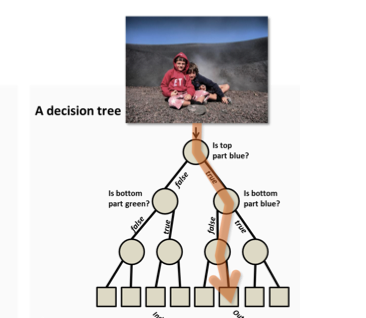
\includegraphics[width=0.6\linewidth]{decisiontree.png}
	\caption[decision tree]{\label{fig:decisiontree}} A decision tree that determines if the picture is taken outdoor or indoor. \cite{DFMS} 
\end{figure}

\subsection{Tree training}
\label{subsec:TTraining}

\begin{figure}
	\centering
	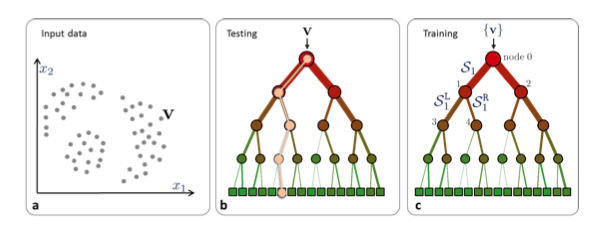
\includegraphics[width=0.6\linewidth]{treeTestTrain.png}
	\caption[Decision tree for 2D data]{\label{fig:treetesttrain}} Decision tree for 2D data clustering\cite{DFMS} 
\end{figure}

Building a tree is a supervised learning problem which requires the training data to be annotated with labels on the target value. For example, input data is in the form of $ \{ (\mathbf{x}_{i},y_{i})\}$, where $\mathbf{x}$ is in 2$\mathbf{D}$ space, $i$ is data label from 1 to $N$ and $y$ is the target value for $\mathbf{x}$.We want to construct the tree which can give the best representation for the associated data. Every data point is sent to the root node and the split function is chosen so that the information gain (discussed later in section \ref{subsec:EIG}) of that split is maximized.(as shown in Figure \ref{fig:treetesttrain} )This process is repeated after each split with the data at each child node until a leaf node is created according to some predefined stopping criteria such as the maximum depth of the tree,etc. \cite{DRFHP}

\subsection{Entropy and information gain}
\label{subsec:EIG}

\begin{equation}
\label{eq:information gain}
	I=H(S) - \sum_{i \in \{1,2\}} \frac{\abs{S^{i}}}{\abs{S}}H(S^{i})
\end{equation}
Equation \eqref{eq:information gain} shows the relationship between entropy and information gain when building a decision tree. Where $\mathit{I}$ is the information gain, $\mathit{H(S)}$ is the entropy of the parent node, $\sum_{i \in \{1,2\}} \frac{\abs{S^{i}}}{\abs{S}}H(S^{i})$ is the expected entropy of its children. As shown in figure \ref{fig:IG}. \textbf{a} is the data set before first split, \textbf{b,c} are the data set after two different splits. And the split in \textbf{c} has a higher information gain than the split in \textbf{b}. This is the most general version of the information gain. However, the measures of entropy  in different problems could vary a lot (discussed in later chapters).

\begin{figure}
	\centering
	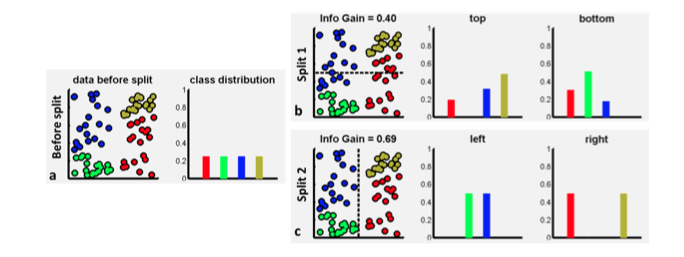
\includegraphics[width=0.8\linewidth]{InformationGain.png}
	\caption[Information Gain for discrete, non-parametric distributions]{\label{fig:IG}}  \textbf{Information Gain for discrete, non-parametric distributions} \cite{DFMS}
\end{figure}


\clearpage
\subsection{Random Forest}
\label{subsec:RF}


A random forest an ensemble of randomly trained decision trees with randomized collection of features at each split \cite{DFMS}.

In general, random forest is distributed algorithm which means that trees are trained in parallel. Compared to other methods such as boosting, random forest has the advantage of searching only in a subset and because of the reduced size of the tests set for each tree, faster training time can be obtained and the collection of the trees at testing time is proved to be more accurate in prediction. Trees in a random forest are learned from randomly sampled subsets of data which reduces over-fitting compared to training on the whole data set. \cite{GFRF, MVDT,RFML} The other randomness which is often used during the training stage of the random forest is a random subset of splits for optimizing the information gain at non-leaf nodes\cite{GFRF}. And overfitting can be avoided by setting the maximum depth of the tree at the beginning. 

At testing time, unseen data is pass to all trees in the forest during which binary test at each node of every tree is performed until the leaf node is reached. After the process, the forest will gather all class distributions of the leaves and produce an average value for the estimation as described in \eqref{eq:randomforestclassification}. Where $ \probability{P}(c|\mathbf{v})$ is the average probability of data point \textbf{v} belonging to class \textbf{c} and $\mathbb{P}_{t}(c|\mathbf{v})$ is the probability of data point \textbf{v} belonging to class \textbf{c} in one tree.
\begin{equation}
\label{eq:randomforestclassification}
	\probability{P}(c|\mathbf{v}) = \frac{1}{T}\sum\limits_{t=1}^T \mathbb{P}_{t}(c|\mathbf{v})
\end{equation}
This the most general version of random forest. There are variations regarding to this report such as the goal of the forest where not classification but regression is needed. These variations will be discussed along with the implementations in the later chapters.


%Head Pose
\chapter{Head Pose Estimation}
\label{sec:HPestimation}

\section{Approach}
\label{sec:HPapproach}

\section{Random Forest Training}
\label{sec:RFtraining}

\subsection{Sample Patches Around Head}
\label{sec:Aroundhead}

\subsection{Dataset}
\label{subsec:HPdataset}

\subsection{BinaryTest At Tree nodes}
\label{subsec:binarytest}

\subsection{Measure of Entropy}
\label{subsec:measureofentropy}

\subsection{Information to be stored at leaves}
\label{subsec:leafdistribution}


\section{Evaluation}
\label{sec:HPevaluation}



%Face feature
\chapter{Facial Feature Points Detection}
\label{sec:FFPD}

The second part of this report will focus on robust face feature detection for 2D images. As far as the method is concerned, again a regression forest similar to the one is used for the head pose estimation with a few variations will be built for purpose. In addition, a robust face detector \cite{facedetect} is also used as a prior step for landmark detection. Although, face detection is not exactly in the scope of this project, some of the necessary details for this algorithm will be mentioned in this chapter. Forest training will be discussed in \ref{sec:FT} and evaluation will be done in \ref{sec:FFeval}.

\clearpage
\section{Face Detection}
\label{sec:FD}
As a preliminary step for feature points detection, face detection is needed since feature points are local information which can only be found around the face area. Haar feature based classifiers are trained to form a such detector.

Firstly, for training images, both positive and negative images are needed. And referencing to sections \ref{sec:HLfeatures} and \ref{sec:integralimage}, rectangular features are calculated from sub windows extracted from each image. Since this pool of candidate features is very big, Adaboost is used to select the best features. \cite{facedetect}

For testing, the most area of an image is non face, we don't want apply every feature selected by Adaboost on every sub windows from test image. Therefore, Viola and Jones "introduce a method for constructing a cascade of classifiers to get good detection rate and decrease the computation time. The idea is to use classifier with less but efficient features to reject the majority of the sub-window before apply more complex classifiers". \cite{facedetect} The two features they used can be seen in Fig \ref{fig:strongclassifiers}. With the filtering procedure, time taken for processing each image is lower. The graphical description of such process can be seen from Fig \ref{fig:cascade}.

\begin{figure}
	\centering
	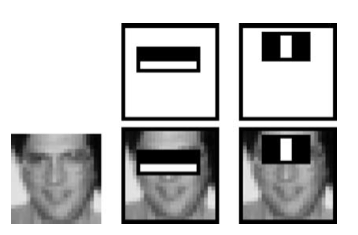
\includegraphics[width=0.8\linewidth]{facedetection.png}
	\caption[Two Efficient Selected by AdaBoost]{\label{fig:strongclassifiers}}  \textbf{"The two features are shown in the top row and then overlayed on a typical training face in the bottom row. The first feature measures the difference in intensity between the region of the eyes and a region across the upper cheeks. The feature capitalizes on the observation that the eye region is often darker than the cheeks. The second feature compares the intensities in the eye regions to the intensity across the bridge of the nose." \cite{facedetect}}
\end{figure}

\begin{figure}
	\centering
	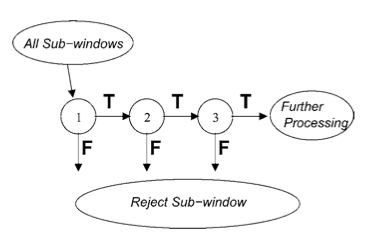
\includegraphics[width=0.8\linewidth]{cascade.png}
	\caption[Cascade Rejection]{\label{fig:cascade}}  \textbf{All sub windows are passed to the cascade of classifiers and in the early stages, the majority of sub windows will be rejected by the initial classifiers and fewer will be left for further processing  \cite{facedetect}}
\end{figure}

\newpage
\thispagestyle{plain}
\mbox{}

\section{Forest Training for Feature Detection}
\label{sec:FT}
Similar to the forest built in chapter \ref{sec:HPestimation}, trees are learned from randomly chosen subsets of all training images. a frontal face detector \cite{facedetect}(implemented by opencv as CascadeClassifier) is used to extract the face bounding box from the given image. Squared patches  $P = ( \alpha^{1},\alpha^{2} ,\theta )$ which are again marked positive and negative are randomly extracted within such bounding boxes and outside the box. Where $\alpha^{1}, \alpha^{2}$ are the image features used, which in this case is the grey values of the raw test images and the normalised grey values to compensate for illumination changes respectively as suggested by \cite{2dGFRF} and $\theta$ is the offset from each feature point to the centre of the patch. 

A pool of binary tests applied to patches at each non-leaf node is the same as did in section \ref{subsec:binarytest} by using equation \refeq{eq:binarytest} with different sub rectangular regions and thresholds. And Each node will split patches into two subsets, namely left and right as before.

Maximizing the information gain \refeq{eq:diffentropy} is required in order to find the best split in the pool. The measure of entropy $H{P}$ would be different from the one used in \ref{subsec:measureofentropy}. Since there are numbers of feature points to be located, $H_{r}(P)$ could be treat as the class uncertainty measure and it is defined as the following: \cite{2dGFRF}
\begin{equation}
\label{eq:classuncertainty}
H_{r}(P) = -\sum\limits_{n=1}^N \frac{\sum\nolimits_{i}p(c_{n}|P_i)}{|P|}log(\frac{\sum\nolimits_{i}p(c_{n}|P_i)}{|P|})
\end{equation}

\begin{equation}
\label{eq:classaffiliation}
p(c_{n}|P_i) \propto exp(- \frac{|d_{i}^{n}|}{\lambda})
\end{equation}

Where $p(c_{n}|P_i)$ is the probability of a given patch ${P_i}$ belongs to the feature point n, which is based on the distance between the patch centre and each of the landmark position. \cite{2dGFRF} And is proportional to $exp(- \frac{|d_{i}^{n}|}{\lambda})$.  Since we still need to classify each patch during testing at the leaf nodes, a measure of the class uncertainty is required. The measure $H_{c}(P)$as described in equation \refeq{eq:cumeasure} is used here. Same as the head pose estimation, $H_{c}(P)$ and $H_{r}(P)$ are combined by a weighted sum as in equation \refeq{eq:okada}. The best test parameters found will be store for each non leaf node.

The objective of forest in chapter \ref{sec:HPestimation} is to predict the location of the nose tip, whereas in this case, there are dozens of landmark locations to infer. Therefore at leaf nodes, the mean and trace of covariance matrices of the offsets to each feature points have to be store.

\newpage
\thispagestyle{plain}
\mbox{}

\section{Evaluation}
\label{sec:FFeval}
The dataset used for this experiment is FaceWarehouse \cite{facewarehouse}. There are 150+ test subjects and each of which has 20 different images taken with various facial expressions. 74 facial landmarks are annotated with each image. 17 of the facial landmarks such as eye brows, nose, eyes, and mouth were chosen for the purpose of this experiment as shown in Fig \ref{fig:expimage}. Image resolution is 640 $\times$ 480. And the faces in this dataset are all frontal faces.

During training, a frontal face detector \cite{facedetect}(implemented by opencv as CascadeClassifier) is used to extract the face from the given image. (shown in Fig \ref{fig:boundingbox}). Once the face bounding box is obtained, random patches with size of 80 $\times$ 80 (same size as used for head pose estimation) are extracted according to the bounding box. Number of patches sampled per training image is 80, one quarter of which are negative patches sampled outside the bounding box and the rest is positive patches. The $\lambda$ in equation \refeq{eq:classaffiliation} is set to 0.125 for this experiment as suggested by \cite{2dGFRF}. 

During testing, for each input image, face is initially extracted to obtain the bounding box ,in which test patches are densely sampled. Each patch is then passed to the trees in the forest where binary tests are performed at each non leaf node with the parameters stored during training. Once the patch reaches the leaf node, the two necessary conditions for a patch to cast a vote for the location of each feature point are as follows. Firstly, the class probability at that leaf node has to be 1 since with the distortion of negative patches, the distribution stored at leaf node is less informative. Secondly, for every leaf node, trace of covariance matrices for each feature point are stored during training, if such trace exceed certain threshold, the patch will not be allowed to cast a vote for the corresponding feature location. The remaining candidate votes are then filtered by mean shift to remove outliers in order to produce the final estimate.

The successful detection for a feature point is determined by whether the estimated point is within a certain region of the actual point. Such region is define by a circle centred at the ground truth point with a radius of 8 pixels as shown in figure \ref{fig:successregion}. Examples of false detection and true detection are shown in figures \ref{fig:fail} and \ref{fig:success}.


\begin{figure}
	\centering
	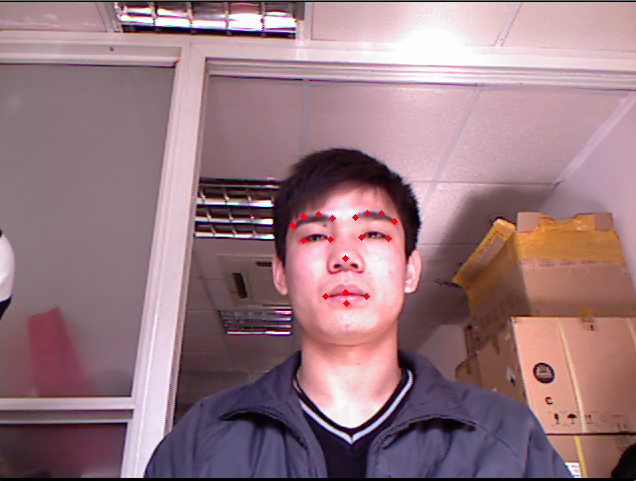
\includegraphics[width=0.8\linewidth]{Screenshot3.png}
	\caption[Landmarks chosen for experiment]{\label{fig:expimage}}  \textbf{Example of an image used for feature points detection, landmarks are marked in red }
\end{figure}

\begin{figure}
	\centering
	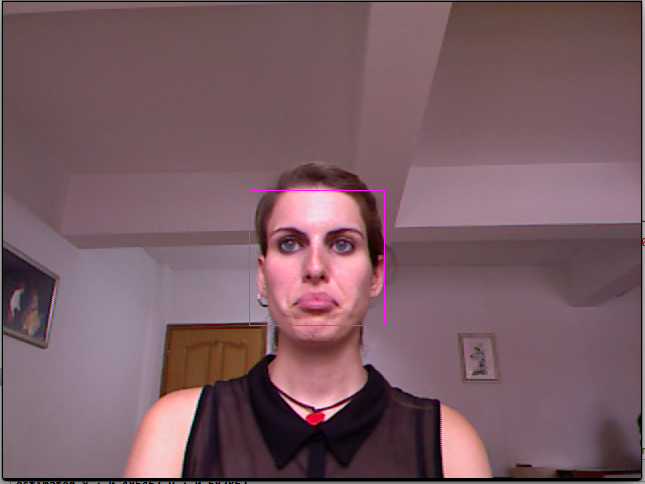
\includegraphics[width=0.8\linewidth]{boundingbox.png}
	\caption[Face detection]{\label{fig:boundingbox}}  \textbf{The region inside the purple bounding box is extracted face }
\end{figure}

\begin{figure}
	\centering
	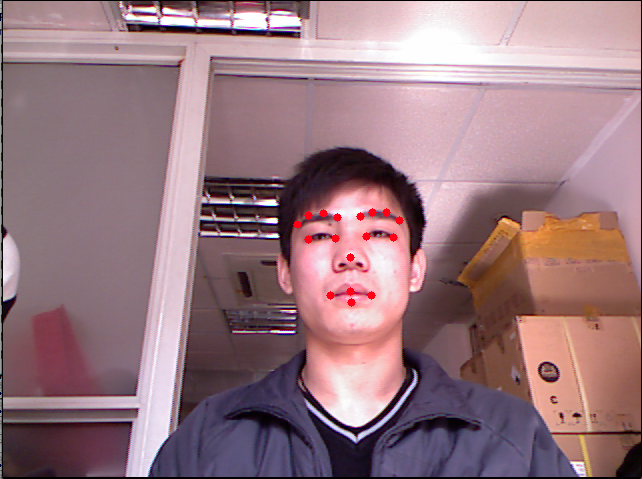
\includegraphics[width=0.8\linewidth]{Screenshot6.png}
	\caption[Landmarks Success Region]{\label{fig:successregion}}  \textbf{The red circles are the error tolerance region for each feature point}
\end{figure}

\begin{figure}
	\centering
	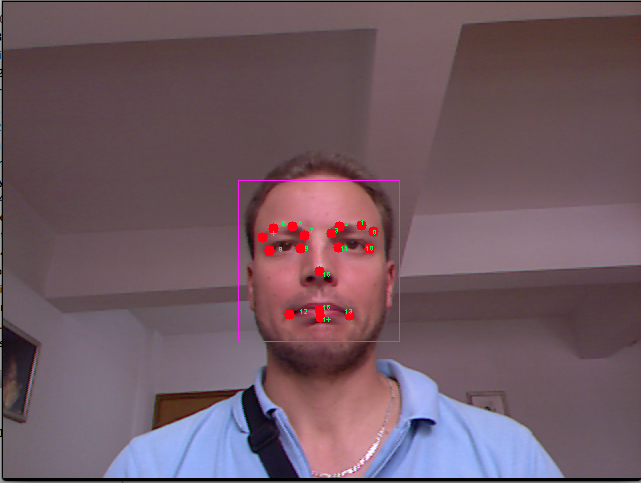
\includegraphics[width=0.8\linewidth]{fail.png}
	\caption[False Detection]{\label{fig:fail}}  \textbf{Example for false detection for some feature points such as points near right eye brow}
\end{figure}

\begin{figure}
	\centering
	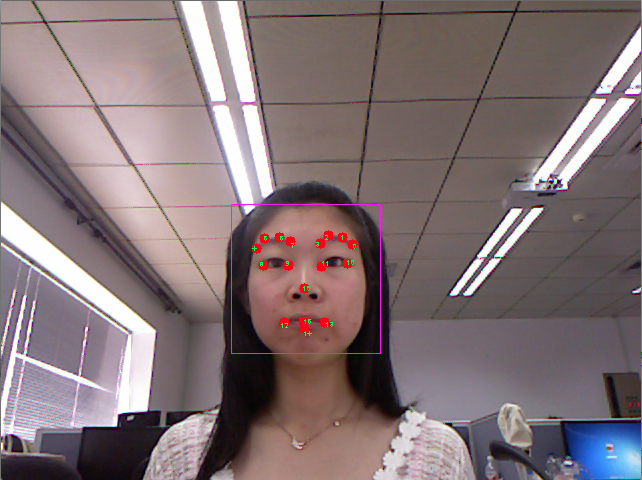
\includegraphics[width=0.8\linewidth]{success.png}
	\caption[Success Detection]{\label{fig:success}}  \textbf{Majority of the features are detected within the margin of error}
\end{figure}

For this experiment, 10 trees are trained and as the number of tree loaded, the accuracy improves as expected as can be seen from the plots \ref{fig:eyebrows},\ref{fig:eyes} and \ref{fig:noseandmouth}. Overall, success rate of feature points around eyes and nose area is higher than the detection rate around mouth. The reason for such low performance around mouth area might due to the huge deformations. When patches are sampled at a density of 5 stride, the overall accuracy is about  3\% higher than when sampled at 10 stride. 

\begin{figure}
        \centering
	 \begin{subfigure}[b]{0.5\textwidth}
                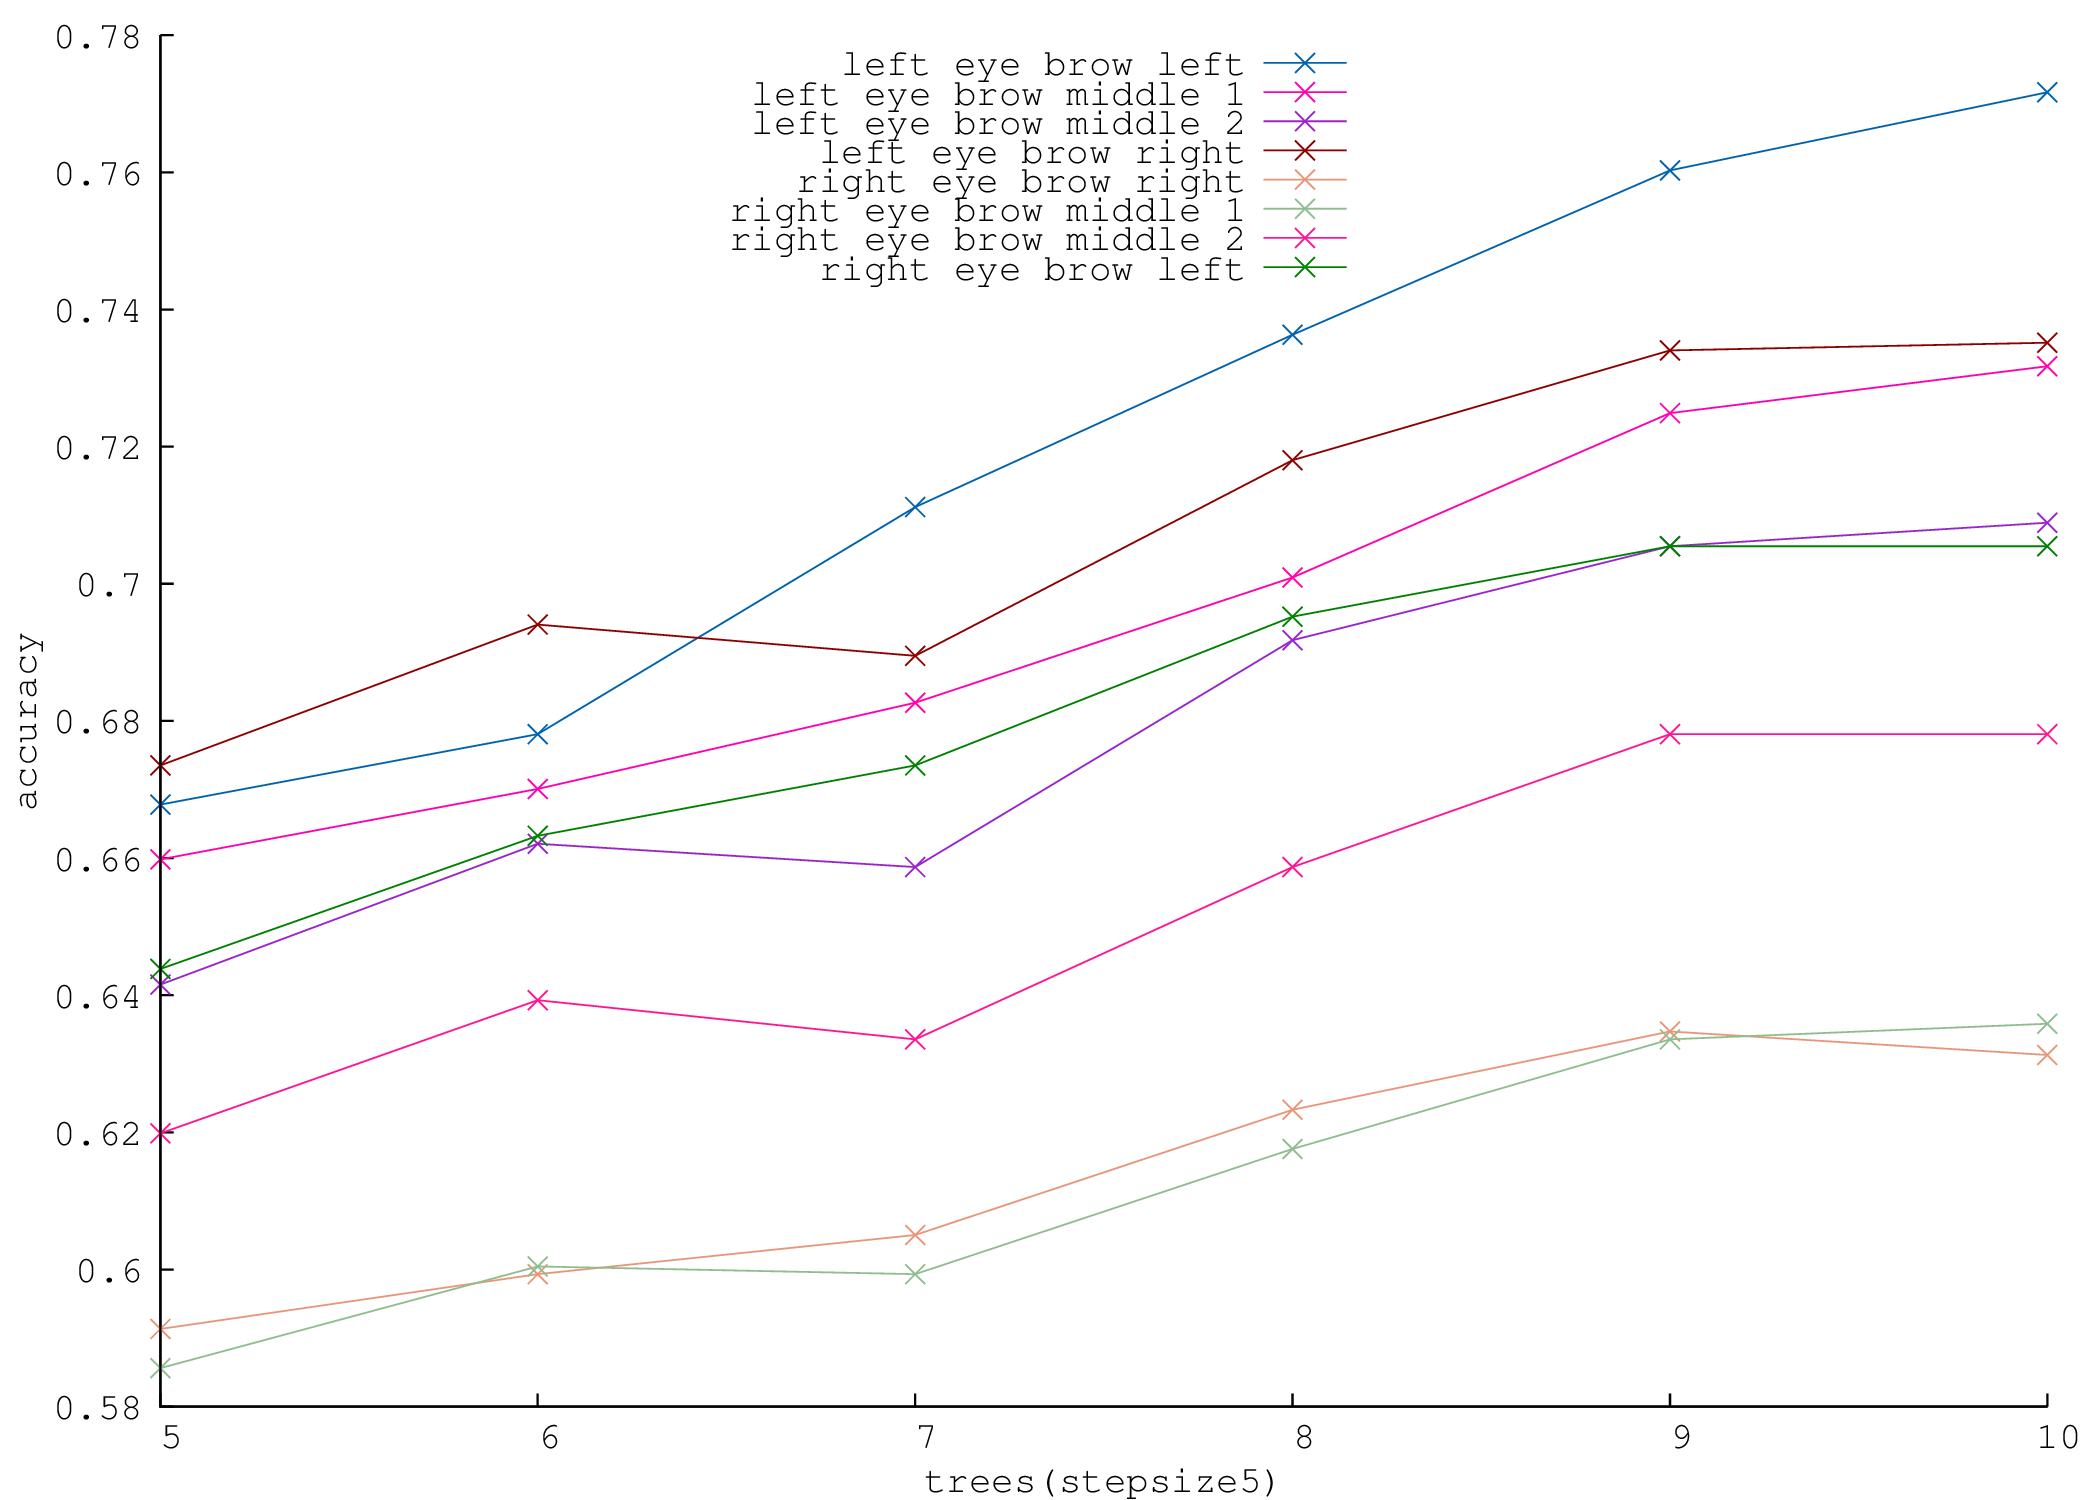
\includegraphics[width=\textwidth]{eyebrowaccuracyvstrees2dss5.png}
                \caption{stride 5}
                \label{fig:eyebrowstride5}
        \end{subfigure}%
        \begin{subfigure}[b]{0.5\textwidth}
                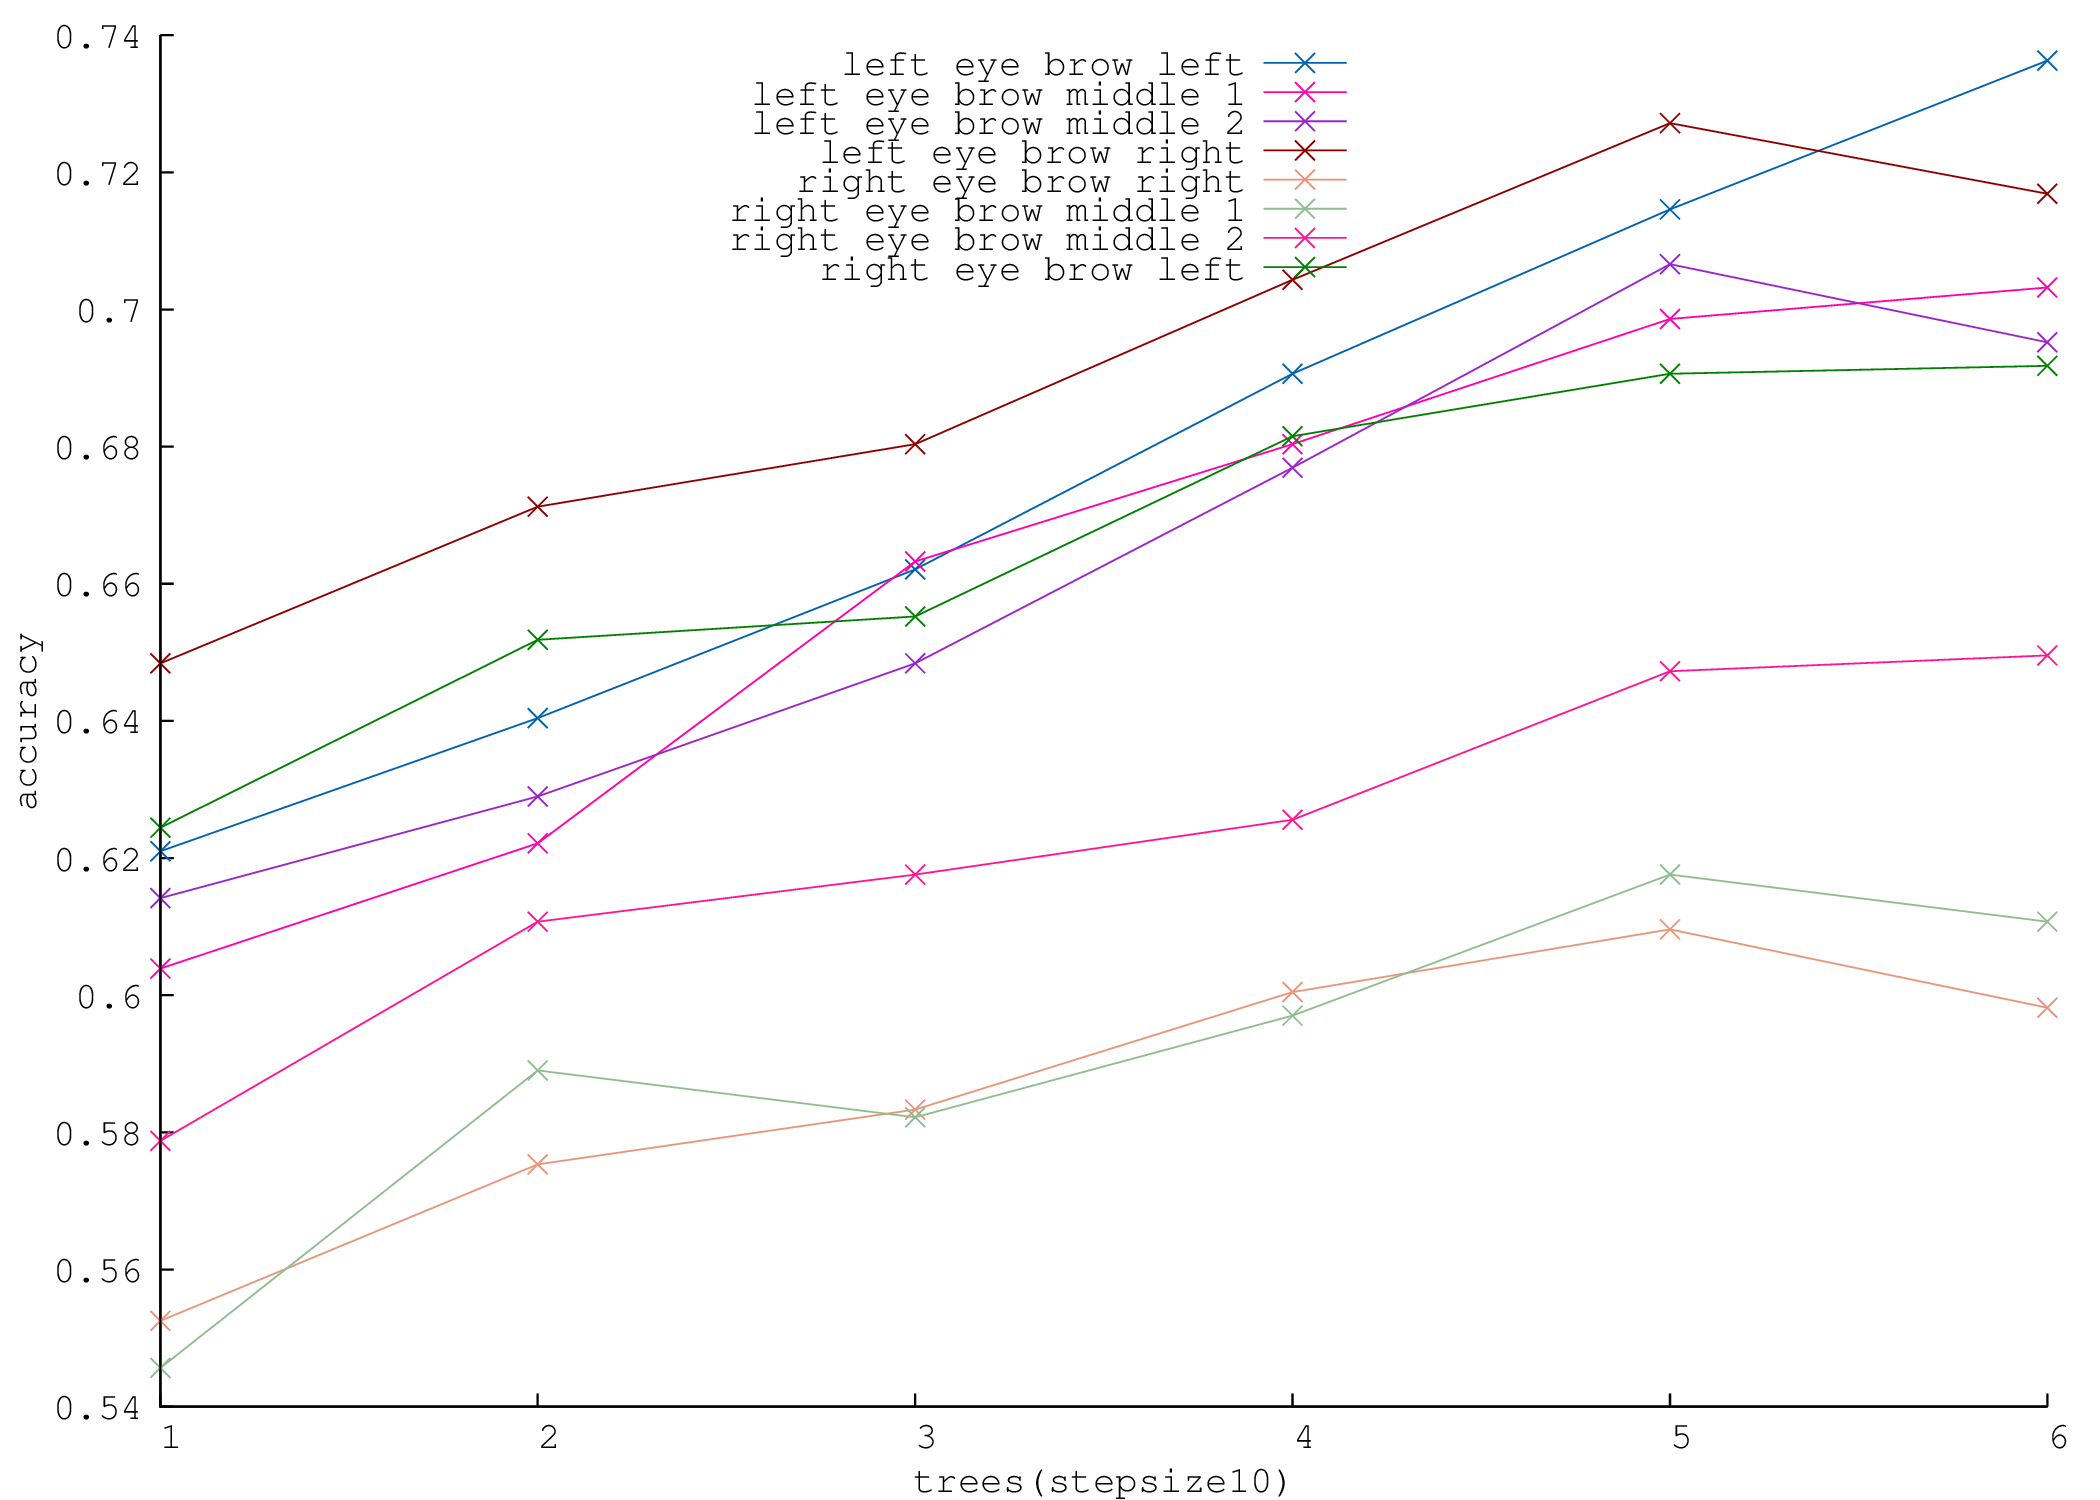
\includegraphics[width=\textwidth]{eyebrowaccuracyvstrees2dss10.png}
                \caption{stride 10}
                \label{fig:eyebrowstride10}
        \end{subfigure}%
        \caption{Eye brows accuracy vs number of trees}\label{fig:eyebrows}
\end{figure}

\begin{figure}
        \centering
	 \begin{subfigure}[b]{0.5\textwidth}
                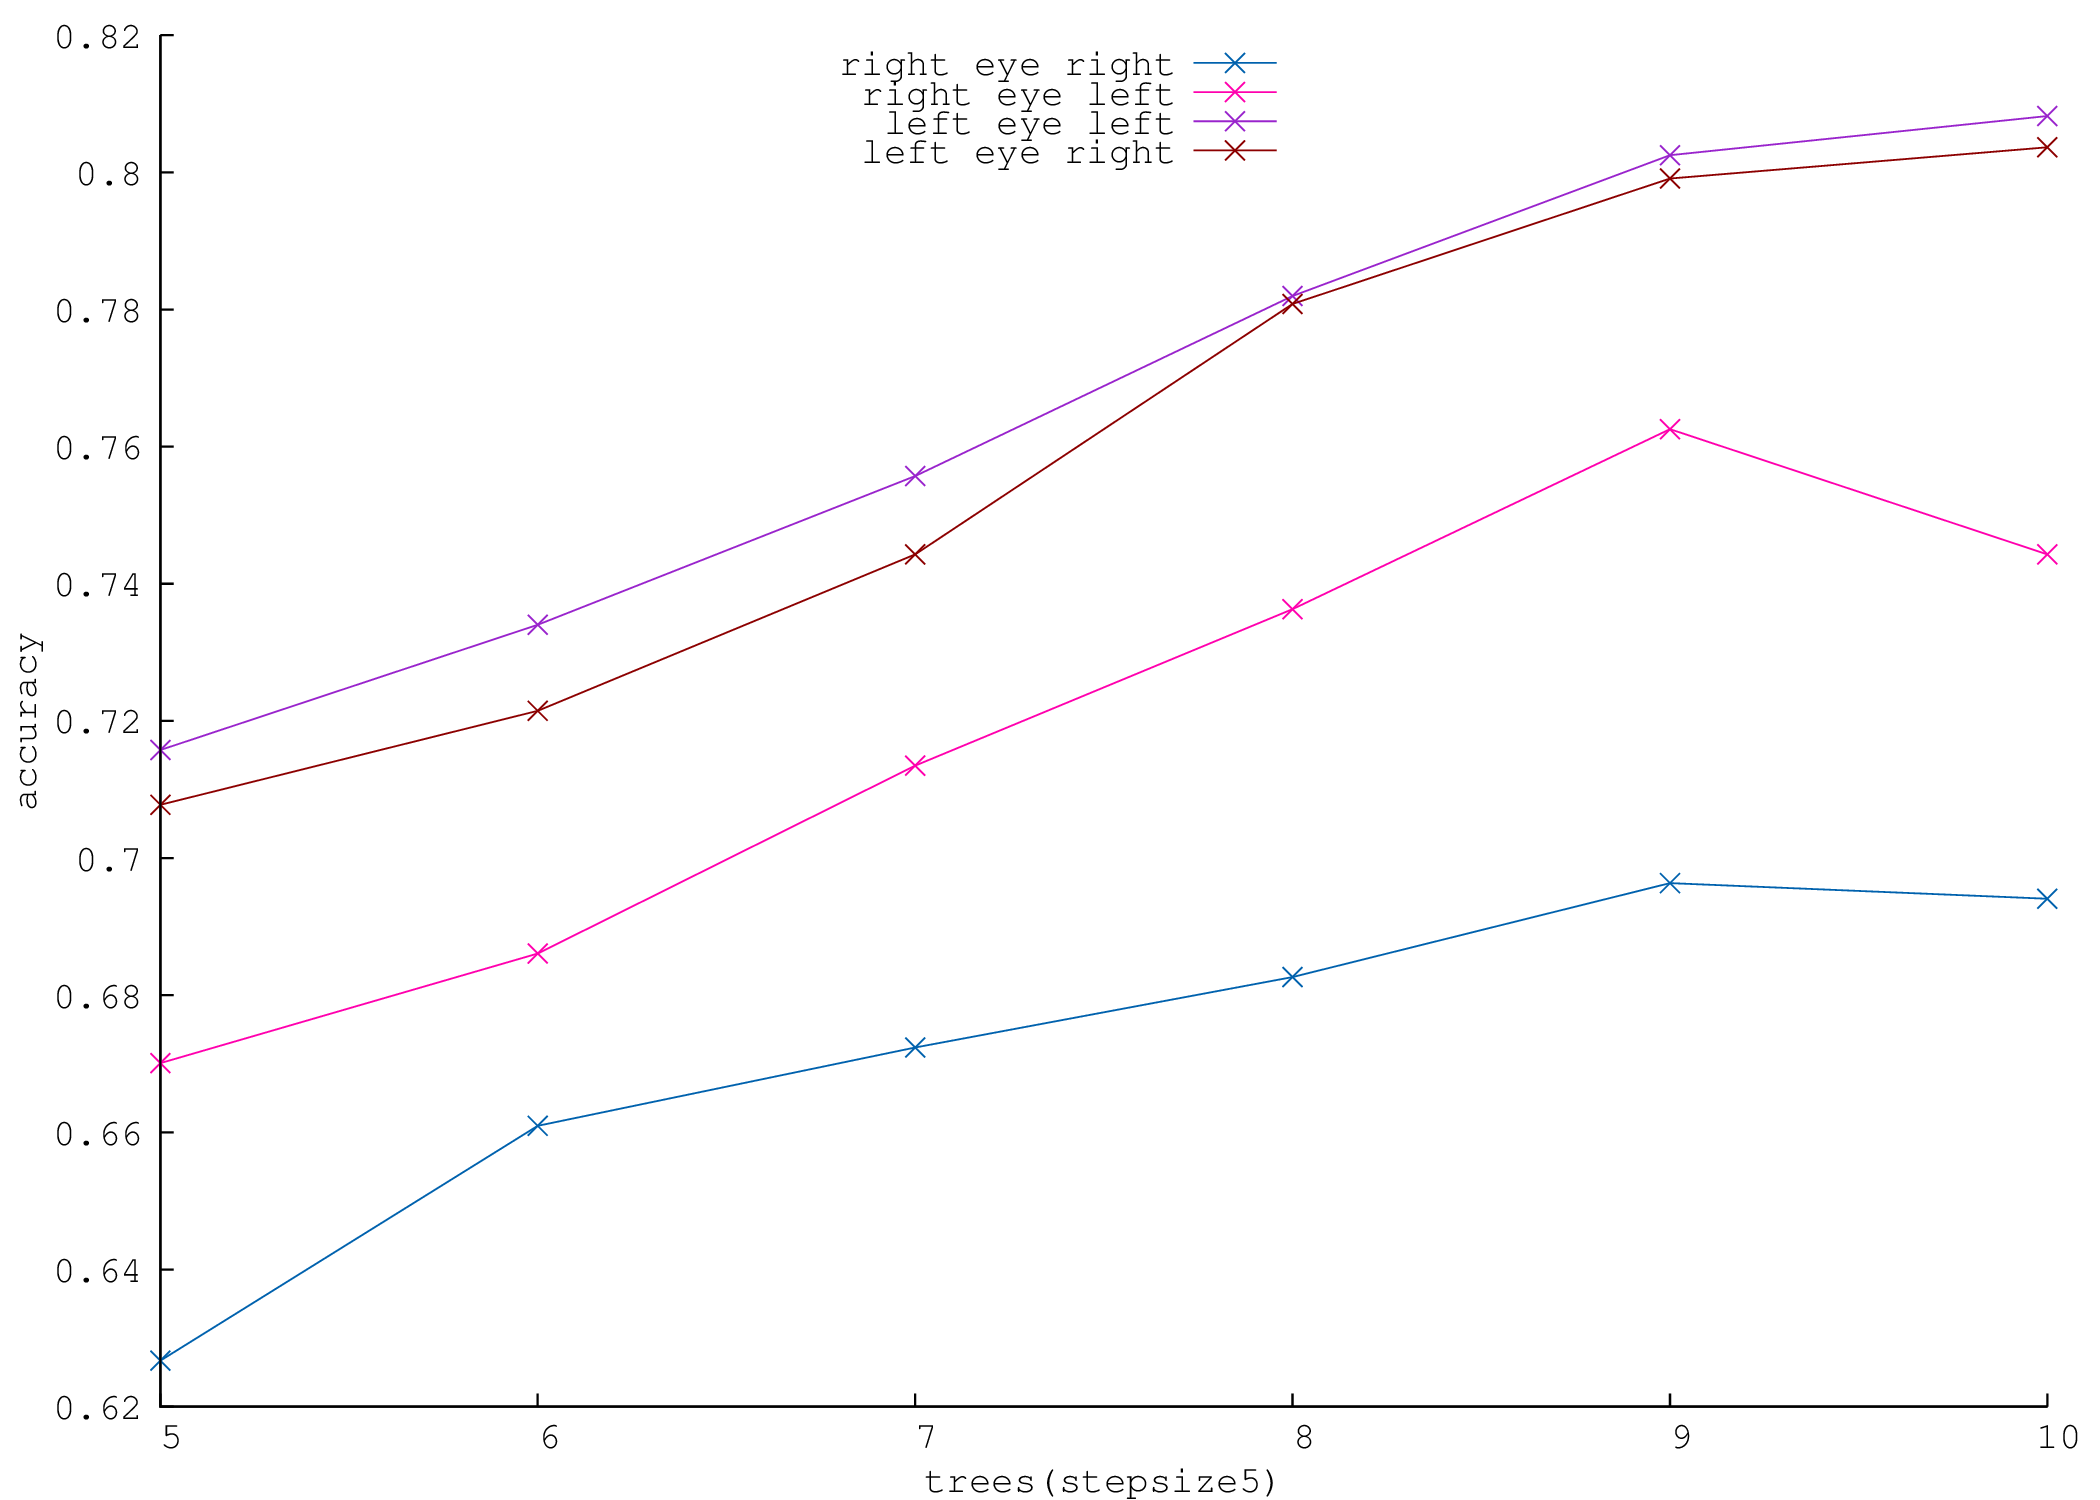
\includegraphics[width=\textwidth]{eyesaccuracyvstrees2dss5.png}
                \caption{stride 5}
                \label{fig:eyesstride5}
        \end{subfigure}%
        \begin{subfigure}[b]{0.5\textwidth}
                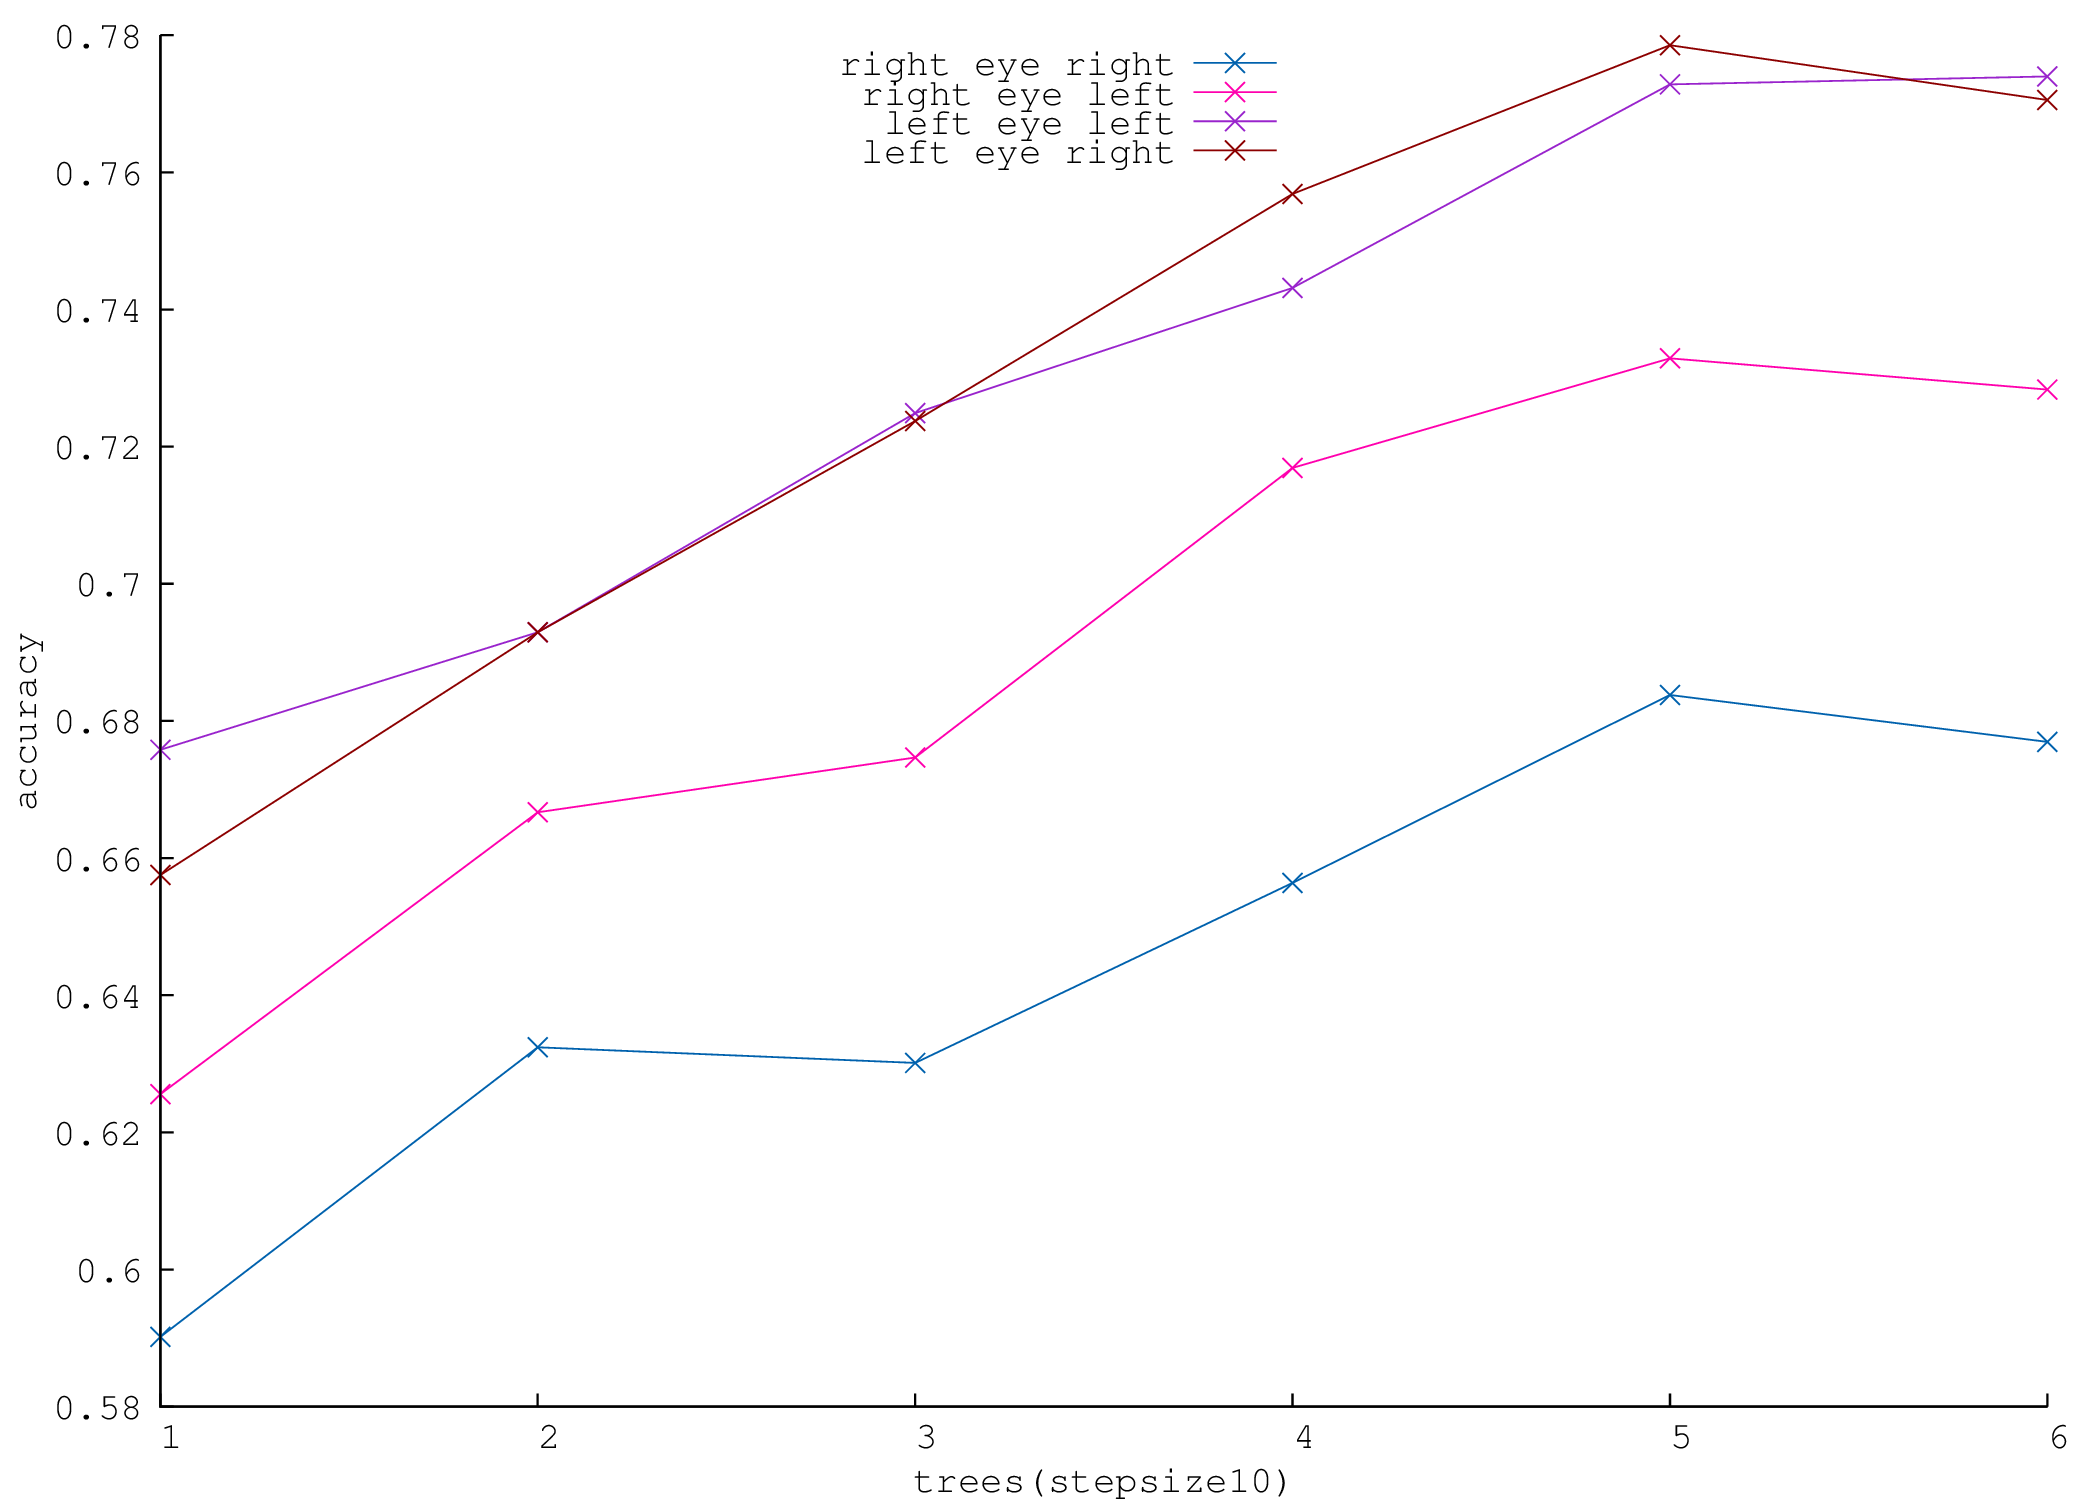
\includegraphics[width=\textwidth]{eyesaccuracyvstrees2dss10.png}
                \caption{stride 10}
                \label{fig:eyestride5}
        \end{subfigure}%
        \caption{Eyes accuracy vs number of trees}\label{fig:eyes}
\end{figure}

\begin{figure}
        \centering
	 \begin{subfigure}[b]{0.5\textwidth}
                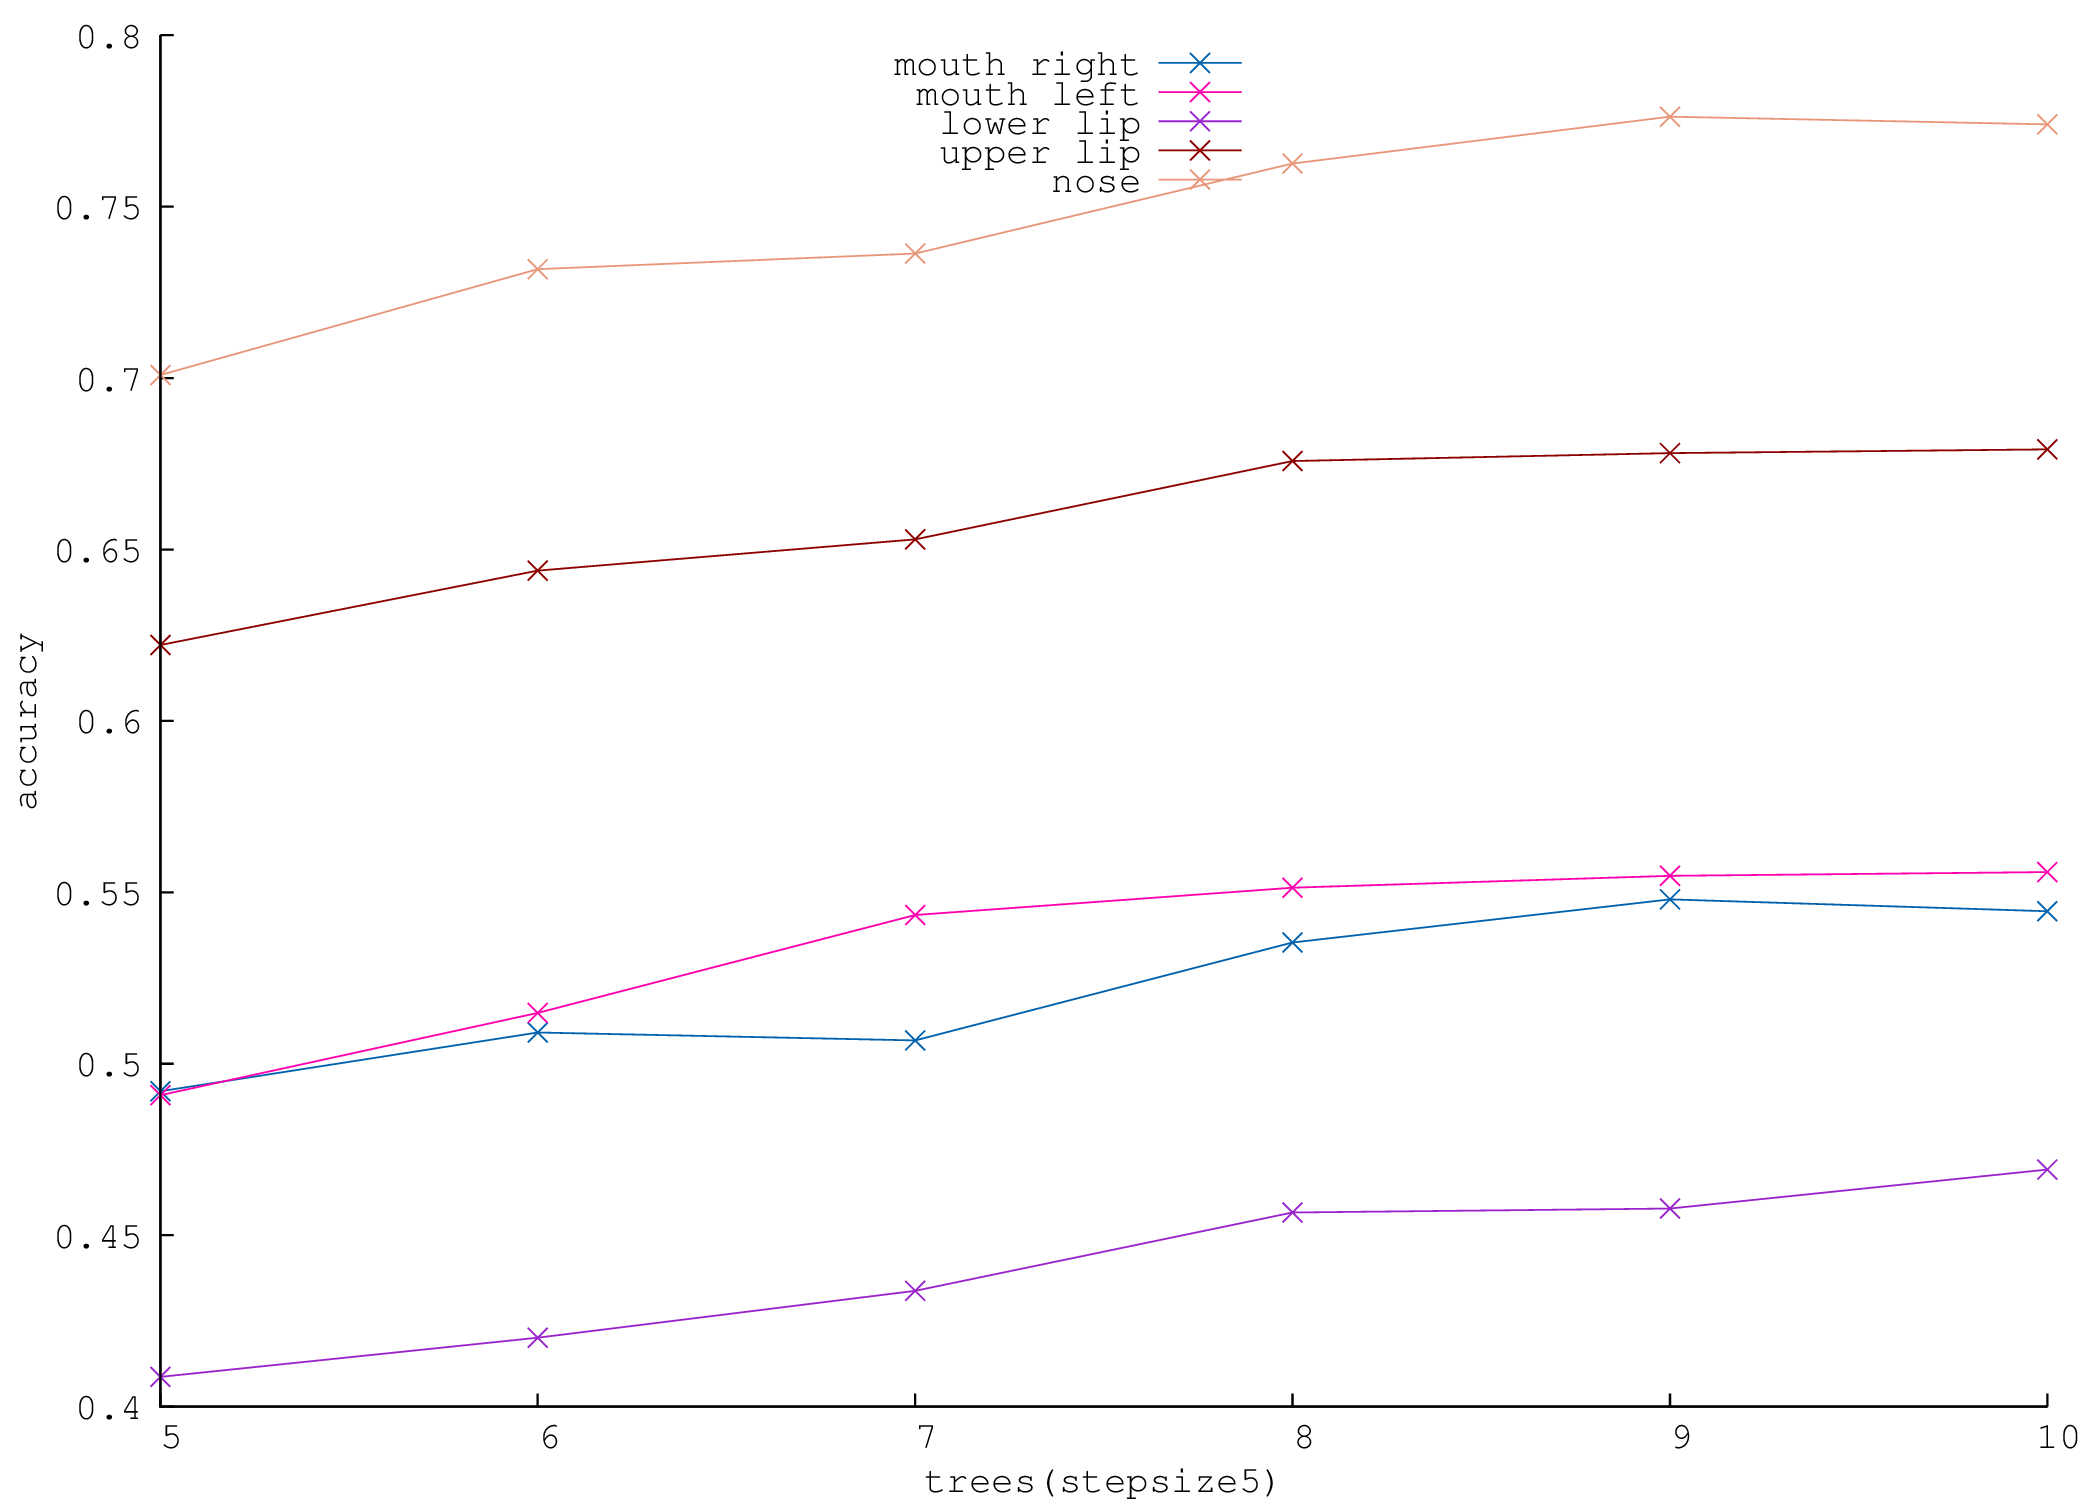
\includegraphics[width=\textwidth]{nosemouthaccuracyvstrees2dss5.png}
                \caption{stride 5}
                \label{fig:eyesstride5}
        \end{subfigure}%
        \begin{subfigure}[b]{0.5\textwidth}
                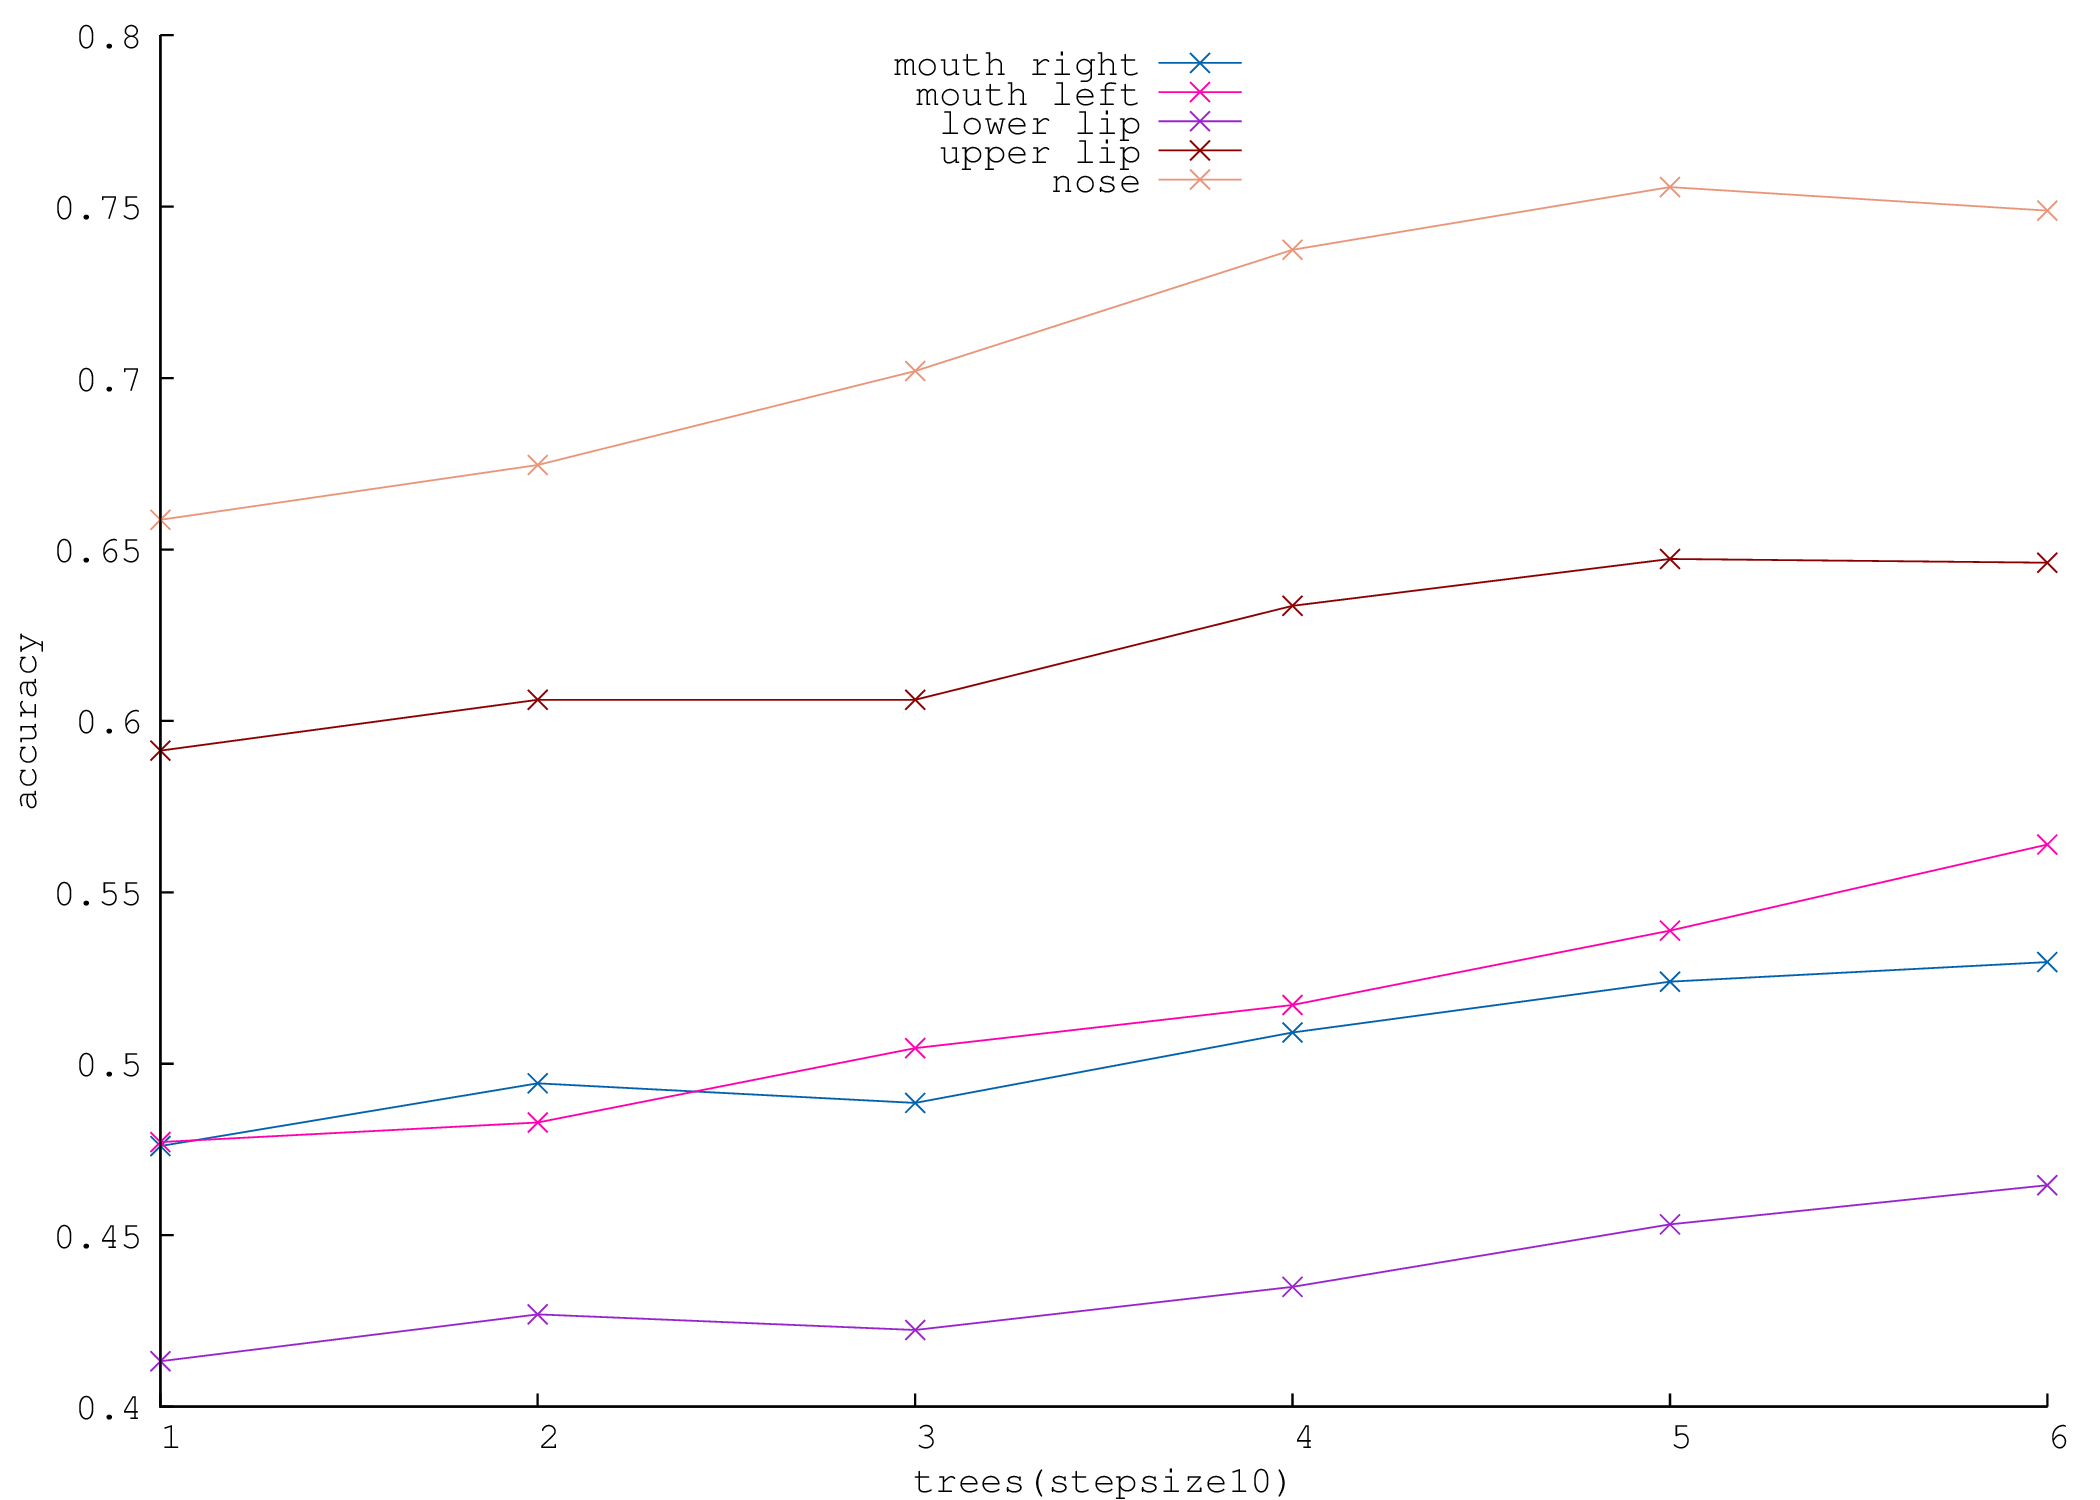
\includegraphics[width=\textwidth]{nosemouthaccuracyvstrees2dss10.png}
                \caption{stride 10}
                \label{fig:eyestride5}
        \end{subfigure}%
        \caption{Nose and mouth accuracy vs number of trees}\label{fig:noseandmouth}
\end{figure}

In addition, speed is also an important parameter in performance and the time taken to process each image is proportional number of patches sampled. Figure \ref{fig:time} shows the relationship between the average time taken to process each image after it has been loaded into memory and the number of trees load. When sampling at a density of 5 stride and 10 trees are loaded, the time taken is approximately 0.1 seconds. In other words, at this sampling density, the system can handle 10 frames per second. However, the computation time decreases to only 0.04 seconds (25 frames per second) when patches are sampled at stride 10 which is a 3 \% drop in accuracy on average.


\begin{figure}
	\centering
	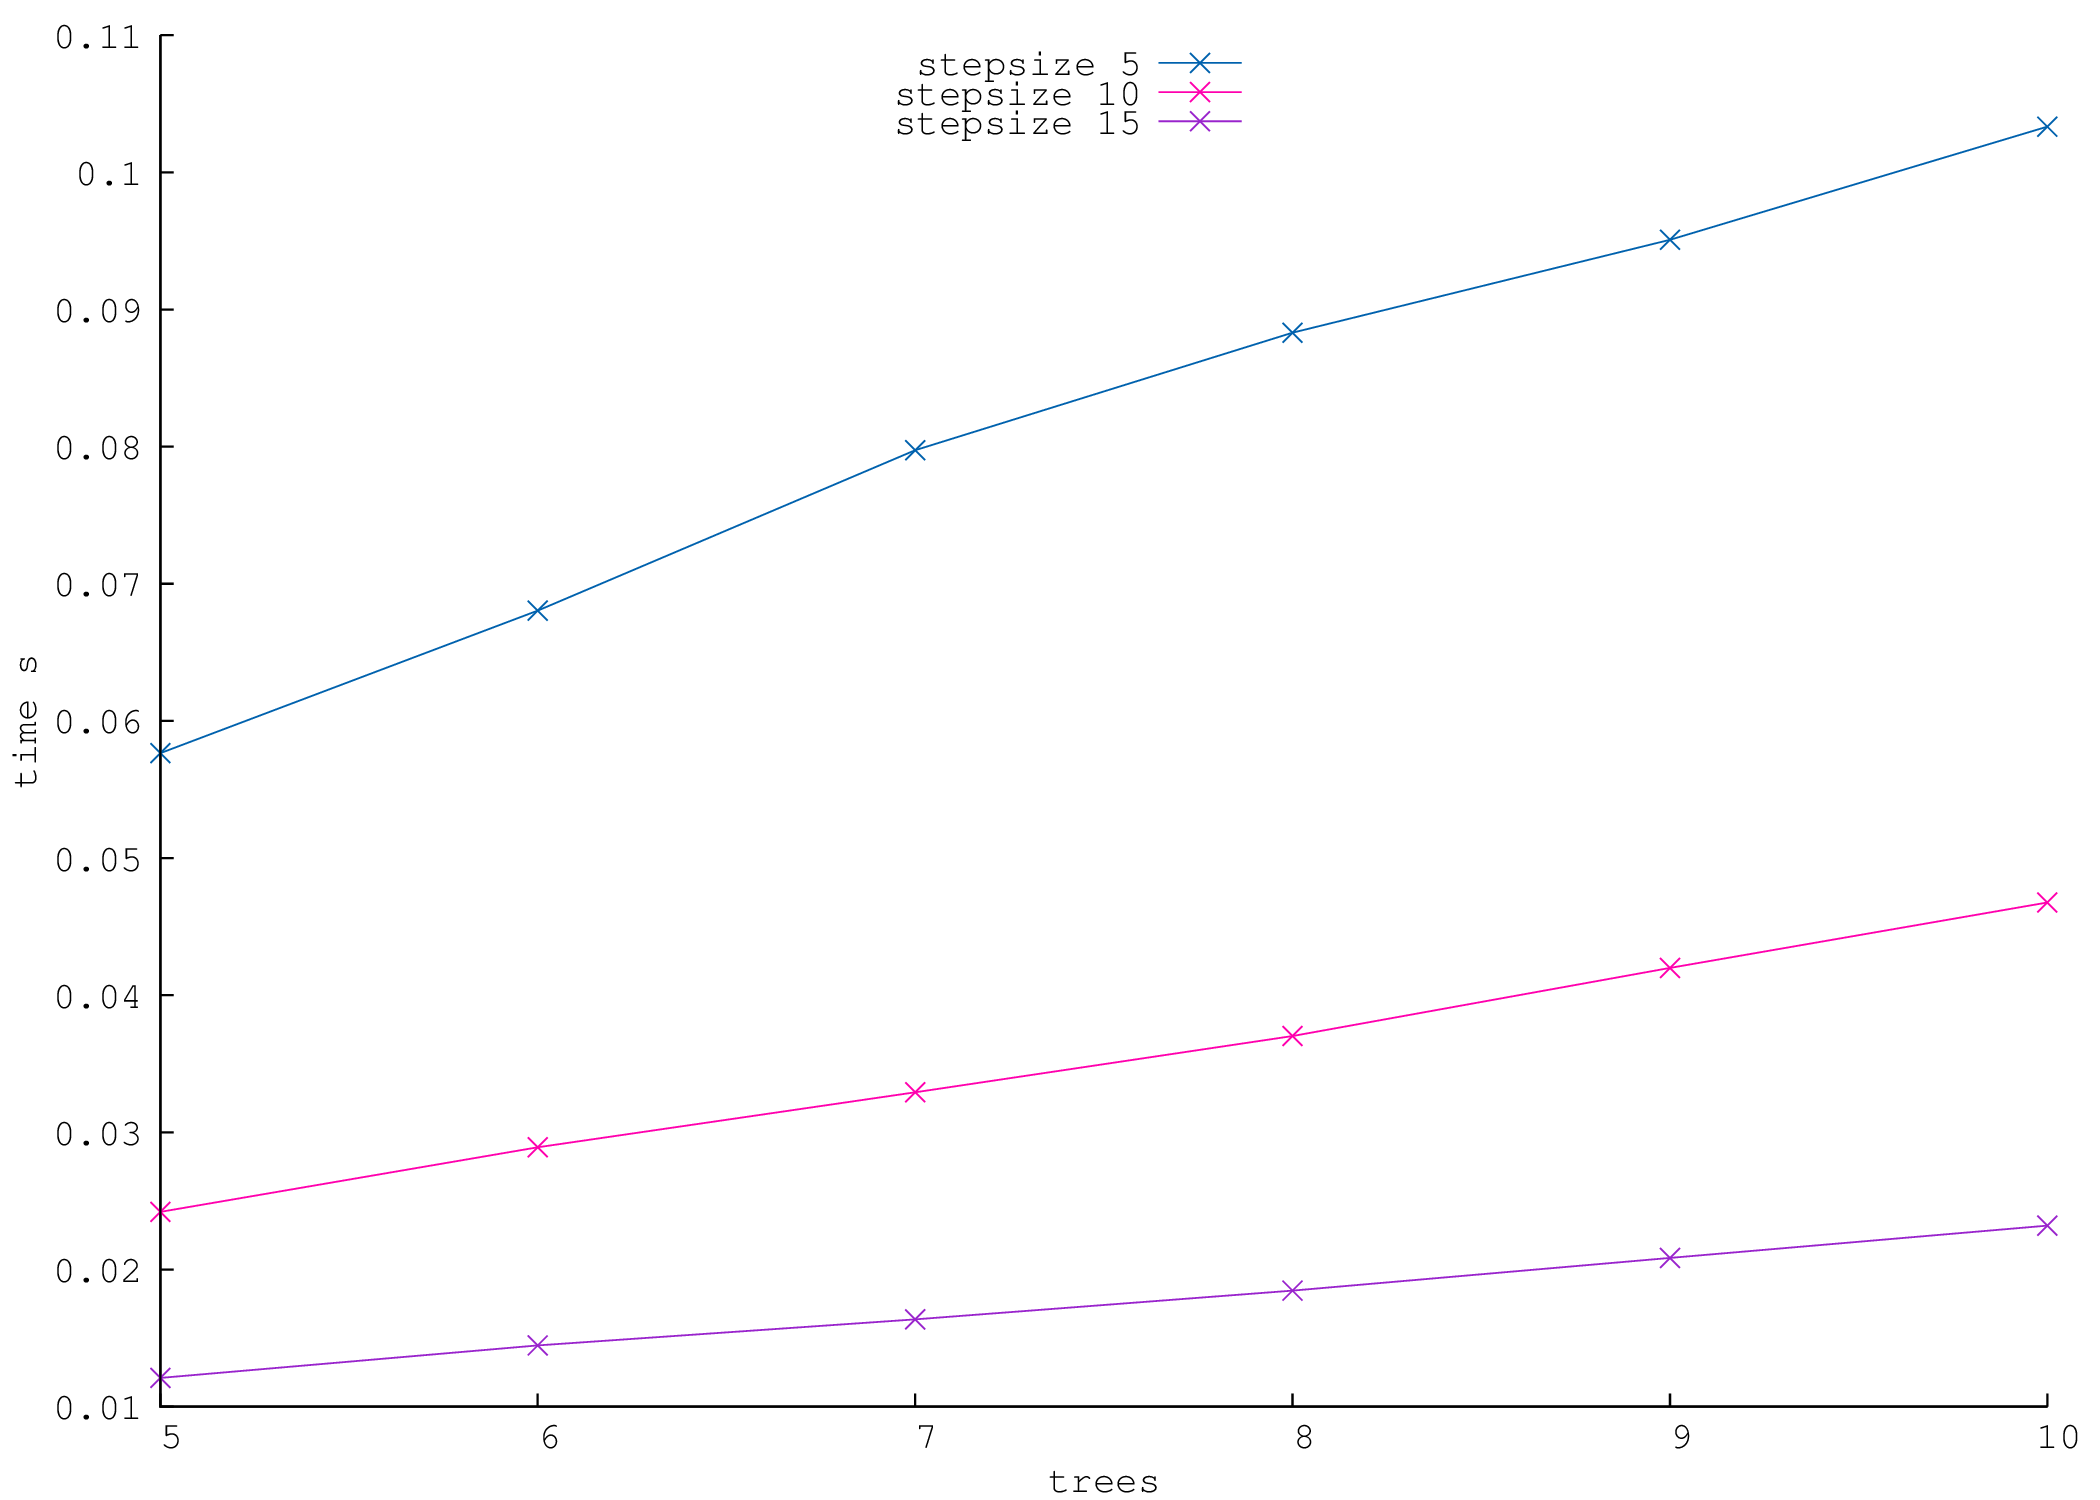
\includegraphics[width=0.8\linewidth]{time.png}
	\caption[Processing time vs number of trees]{\label{fig:time}}  \textbf{average processing time for each image(frame)various densities, stride 5,10,15 in blue,pink,purple respectively }
\end{figure}

%Conclusion
\chapter{Conclusion and Further Work}
\label{section:conclusion}

%----------------------------------------------------------------------------------------
%	THESIS CONTENT - APPENDICES
%----------------------------------------------------------------------------------------

\appendix % Cue to tell LaTeX that the following 'chapters' are Appendices

% List of FTSE 100 Stocks considered
%\input{appendices/appendixA}

\backmatter

%----------------------------------------------------------------------------------------
%	BIBLIOGRAPHY
%----------------------------------------------------------------------------------------

\newpage
\thispagestyle{plain}
\mbox{}
\label{Bibliography}

\bibliographystyle{hieeetr}
\bibliography{}
%%% Add bibliography here
%\bibliographystyle{hieeetr.bst}
%\bibliography{finalbib}

\end{document}  